% \documentclass{article}
\documentclass[platex,a4j,11pt,dvipdfmx]{jsarticle}
\usepackage[utf8]{inputenc}
\usepackage[T1]{fontenc}
% \usepackage[OTF]{fontenc}
\usepackage{geometry}
\geometry{a4paper, margin=1in}
\usepackage[explicit]{titlesec}
\usepackage{needspace}
\usepackage{etoolbox}
\usepackage{tocbibind}
\usepackage{tcolorbox}

\definecolor{stepheadingbackground}{RGB}{232,240,245}
\titleformat{\subsection}[block]
  {\normalfont\large\bfseries}
  {}
  {0pt}
  {\colorbox{stepheadingbackground}{%
    \parbox{\dimexpr\linewidth-2\fboxsep\relax}{%
      \raggedright\strut\thesubsection\quad #1\strut}}}
\titlespacing*{\subsection}{0pt}{3.25ex plus 1ex minus .2ex}{1.5ex plus .2ex}
\pretocmd{\subsection}{\Needspace{6\baselineskip}}{}{}

\usepackage{amsmath}
\usepackage{amssymb}

\usepackage{pre}
%\usepackage{hyperref}



\title{Part II : 統計学}
\title{Part II : 統計学 (第二稿)}
\author{}
\date{}

\begin{document}

\maketitle

\tableofcontents

\newpage

% 第1章 (概観). 本文の五段 (第2〜6章) とは別
\section{統計学的にデータを調べるということ}

  \subsection{運まかせを疑う}

    じゃんけんに負けても, 普通は運が悪かったと思うくらいだろう.
    どの手が出るかは運まかせで, 勝てるのは3回に1回だと思っているからだ.
    ところが, 出した手を何千回も記録してみると, 人の出す手には案外偏りがある.
    ある調査\footnote{%
    芳沢光雄『じゃんけんの算数：樹形図と確率の考えかた』日本評論社, 2006年.
    学生725人・延べ11{,}567回のじゃんけんデータに基づく.
    集計値は長谷実李・青山和裕「じゃんけんの強さとその人の性格特徴の相関性」『日本科学教育学会研究会研究報告』34巻3号, 2019年, 53--58頁, doi:10.14935/jsser.34.3\_53にも再掲されている.}
    によると, グー・チョキ・パーの出た割合はおよそ 35 : 32 : 33 だったそうだ.
    35\%と32\%ならたったの3ポイント差で, ほとんど互角に見える.
    100回くらいのじゃんけんなら, このくらいの差は偶然でもよく出る.
    だが, 11{,}567回も集めた上での3ポイント差となると, これは偶然とは片づけにくい.

    ただ, 実際に勝てるかどうかは別の話だ.
    仮に相手がこの割合のままずっと手を出し続けてくれたとしても, こちらがパーを出し続けて勝てる割合は約35\%.
    相手がまったくでたらめに出すときの約33\%と比べて, 2ポイントほど高いにすぎない.

    さて, ここまでだと「なんだ, たった2ポイントか. もっと勝てる方法はないのか」という感じかもしれない.
    ところが, じゃんけんを何回か続ける状況を考えると, 様子が変わってくる.
    手がかりになるのは, 相手が直前に何を出したかだ.
    でたらめに出しているなら, 1回目と同じ手を2回目にまた出すのは3回に1回のはずだ.
    同じ人が2回続けてじゃんけんをした10{,}833組の記録を見ると, 1回目と同じ手をまた出したのは2{,}465組で, 約23\%しかなかった.
    たとえば, グーであいこになったとしよう.
    相手がこの傾向どおりに手を出すとすれば, 次も続けてグーを出してくるのは23\%くらいしかない.
    それなら, こちらはチョキを出せばいい.
    負けるのは相手がもう一度グーを出したときだけだ.
    当てもなく手を出せば $1/3$ の確率で負けるところを, 23\%ほどまで下げられる.

    だから, 自分はグーを出し続けるのだ, という強固な信念がない限り, あいこになった場合はこの傾向に従ってチョキを出すほうがクレバーだといえる.
    このように, 確実にこうだ, ということはわからないが, こうなる可能性が比較的高いぞ, と言うための根拠を与えてくれるのが統計のよいところの一つだ.
    現実は複雑なのでもごもごした物言いになってしまうが, それが統計の味わいというものである.

  \subsection{確率論で扱うサイコロと統計学で扱うサイコロ}

    確率論と統計学はいずれも平たく言うと「物事がどのくらい起こるのか」を考えるものであり, ともするとどんな違いがあるか, 
    はっきりしないと思われるかもしれない.
    これにはいろいろな表現があると思うが, ここでは簡単に, 確率論はより理論的であり, 統計学はより実践的だ, という違いを挙げておきたい.

    たとえば, 手元にサイコロが一つあって, 暇つぶしに（ちょっと寂しすぎる気もするが）20回振ってみたとしよう.
    1の目が出た回数を数えてみると, なんと10回もあった.
    1の目が出る確率は $1/6$ だから, 20回振れば3回か4回程度になるはずだ.
    半分が1というのは, いくらなんでも多すぎる.
    「このサイコロ, 中に重りでも入っているのではないか」と疑いたくなる.

    とはいえ, まともなサイコロであっても, 20回振って1がきっちり3回や4回出るとは限らない.
    1回しか出ないこともあれば, 6回出ることだってある.
    10回出る確率も, 決してゼロではない.
    極端な話をすれば, 20回すべてが1になる確率さえゼロではないのだ.
    1が10回出るという現象は, 細工のあるサイコロでも, ないサイコロでも起こりうる.
    どれだけサイコロを眺めても, どちらか区別できない.
    すると, 1が10回出たという結果から判断するしかないが, これだけでは細工があるとまでは言い切れない.

    もっとも, 20回すべてが1になるような確率まで気にしていたらきりがないが, やはり10回も出るのは怪しい.
    そう感じるのは, 「まともなサイコロなら, そんなに1ばかり出ないはずだ」と思うからだ.
    それなら, まともなサイコロで1が10回以上出るのがどれくらい珍しいことなのかを計算してみよう（ちょうど暇だ）.
    たとえば1が6回程度なら, 「今日はよく1が出るな」くらいで済ませるだろう.
    実際, まともなサイコロを20回振って1が6回以上出る確率は, 1割ほどある.
    ところが10回以上となると, 確率はおよそ1700分の1にしかならない.
    「たまたま」で片づけるには, さすがに珍しすぎる確率だ.

    ただし, この1700分の1という数値は, 「どの目も $1/6$ の確率で出る」とあらかじめ定めた, まともなサイコロを前提に計算したものだ.
    確率論が扱うのはこのようなサイコロであり, 前提となる条件が初めから決まっているため, 正しく計算すると答えはただ一つに定まる.
    一方, 統計学が扱うのは目の前にある実際のサイコロだ.
    その構造が本当に偏りのないものなのかは分からないし, 何回振ったところで完全に確かめることはできない.
    そこで統計学では, 「絶対に細工がある」と断定する代わりに, 「確率が1700分の1という極めて珍しい出来事が起きたか, さもなければサイコロに細工があるかのどちらかだ」と主張する.
    どちらが真実なのかまでは言及しないが, 1700分の1というおかしな数値を聞けば, 誰もがサイコロの仕込みを疑いたくなるだろう.

    アンケートの回答から社会の意見を推し量ることも, 1万回を超えるじゃんけんの記録から人間の癖を探ることも, このサイコロの例と同じだ.
    確率論は, あらかじめまともな作りだと決めたサイコロを出発点として, どの目がどれくらいの割合で出るかといったことを考える.
    反対に統計学は, 実際に目の前にあるサイコロを振って出た目を出発点として, そのサイコロの構造について何が言えるかを探るのだ.
    出た目からサイコロの構造へさかのぼる過程には, どうしても確実と言い切れない部分が残ってしまう.
    このように統計学は, 不確かな部分をあえて言い切らずに残したまま, 目の前のデータがどれほど珍しいのかを確率というグラデーションで表現する.

  \subsection{このパートで学ぶこと}

    このパートでは, 具体的な例を一つずつたどりながら, 珍しさを表す確率がどこから出てくるのか, それをもとに何がどこまで言えるのかを考えていく.
    そうしていくうちに, もごもごした物言いにも, ちゃんとした理屈があることが見えてくるはずだ.
    完全に納得とはいかないまでも, こういう考え方もありだな, と受け入れてもらえれば十分である.

    まずは, データを平均のような一つの数にまとめるところから始める.
    何が珍しいのかを考えようにも, 何の数字について考えるのかが決まっていなければ話にならないからだ.
    手元のデータについて知りたいだけなら, 平均を計算すればそれで終わりだ.
    ただ, 知りたいのはたいてい, 手元のデータよりもっと大きな全体のほうだ.
    アンケートなら, 知りたいのは回答した人たちの意見ではなく, 社会全体の意見だろう.
    ところが, 手元のデータで計算した値は, 当然データを取り直すと別の値になってしまう.
    どのくらい変わるのかがわからなければ, 手元の平均から全体についてどこまで言っていいのかもわからない.
    それでも, 取り直したときに平均がどのくらいばらつくのかは, 手元のデータだけから計算できてしまう.
    このばらつきをもとに, 「全体の平均はだいたいこのあたりだろう」「二つのグループの差はこれくらい珍しい」といったことを確率で表していく.
    もっとも, 差が珍しいとわかっても, なぜその差が生まれたのかまではわからない.
    原因を確かめるには, 計算よりも, どう比較するかのほうが大事になってくる.
    それに, データの集め方が偏っていたら, せっかくの計算も当てにならない.
    そこでこのパートの最後では, データがどうやって集められたのかまでさかのぼって考える.

    推定や検定, 相関といった, 統計学の入門でかならず出てくる話題は, このパートでもひととおり扱う.
    だから, 読み終えたあとで統計学をもう少し深く学ぼうと思ったときにも, ここで扱った話題が足場になるはずだ.


\newpage

% 第2章 = 第1段「何についての数字かが, 言えることを決める」
\section{何についての数か}

  \subsection{平均が同じ二つの商品}

    食事に行く店を決めたり, 通販で家電を選んだりするとき, まず目に入るのはレビューの星だろう.
    星の平均が4.2の製品と3.1の製品が並んでいたら, とりあえず4.2のほうを開いてみる.
    何十人もの評価を足して割った数を見れば, 一件ずつレビューを読まなくてもだいたいの様子がわかるからだ.

    この計算は, 算数で習った平均そのものである.

    \begin{defi}{平均}{mean}
      $n$個の観測値 $x_1, x_2, \ldots, x_n$ に対し,
      \[
        \bar{x} = \frac{1}{n} \sum_{i=1}^{n} x_i
      \]
      を\textbf{平均}（算術平均）と呼ぶ.
    \end{defi}

    式にすると少し構えてしまうかもしれないが, 要するに全部足してデータの個数で割っているだけだ.
    計算も簡単で, どれほどたくさんのデータがあっても一つの数にまとめられる.

    では, 同じ星4.0の製品が二つ並んでいたらどうだろう.
    レビューの件数も気になるところだが, どちらも同じ20件だったとする.
    こうなると, 星の平均だけを見ていてもどちらを選ぶべきか判断がつかない.

    しかたがないので, 4.0という計算のもとになった20件の評価そのものを確認してみよう.
    商品Bについた20件を, 投稿された順に並べてみる.

    \begin{center}
      5, 5, 1, 5, 5, 5, 1, 5, 5, 5, 5, 1, 5, 1, 5, 5, 5, 5, 1, 5
    \end{center}

    これを見てすぐに気づくのは, 5と1しか並んでいないことだ.
    平均は4.0なのに, 4点をつけた人は一人もいない.

    一方の商品Aの20件は次のようになっている.

    \begin{center}
      3, 4, 5, 4, 4, 3, 4, 5, 4, 3, 4, 4, 5, 3, 4, 5, 4, 3, 4, 5
    \end{center}

    こちらは3と4と5が混ざっていて, 4点が多そうだ.
    どちらの商品も, 20件の数字を全部足して20で割ればきっちり4.0になる.
    しかし, 列を眺めただけでは正確に何点が何件あるのかまでは数えにくい.

  \subsection{点数ごとに数え直す}

    そこで, 点数ごとに何件あるのかを数えてみる.
    1点が何件, 2点が何件, と数え直して, 横軸に点数, 縦軸に件数を取って棒の高さで表してみる.
    \cref{fig:ch02-ab}がその図だ.

    % 図のデータ: 仮. 要作成
    \begin{figure}[htbp]
      \centering
      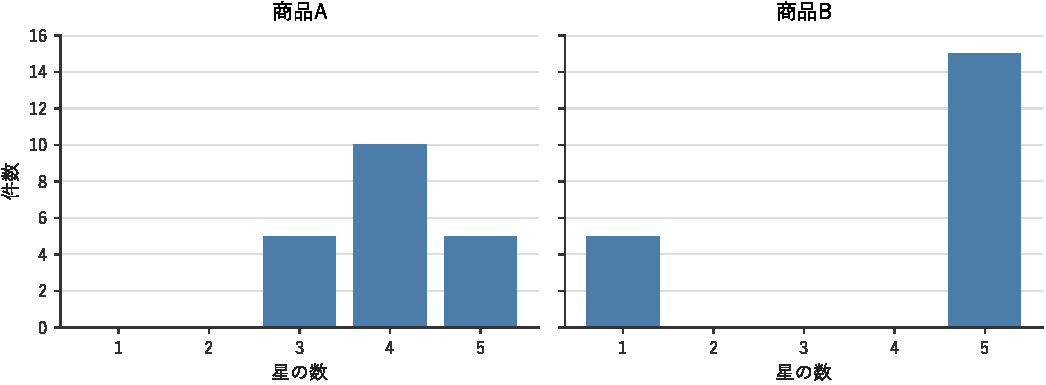
\includegraphics[width=\linewidth]{../figures/output/ch02_ab.pdf}
      \caption{商品Aと商品Bのレビュー20件を, 点数ごとに数えた図. 横軸は星の数, 縦軸は件数. 二つの図で軸をそろえてある.}
      \label{fig:ch02-ab}
    \end{figure}

    こうして並べてみると, 二つの違いがはっきりと見える.
    商品Aは4点が10件あって, その両隣の3点と5点が5件ずつある. 4点を中心にきれいに固まっている.
    これに対して商品Bは, 5点が15件もある一方で, 1点も5件ある. あいだの2点, 3点, 4点は文字どおりゼロだ.

    もちろん, 平均の計算を間違えたわけではない.
    5点が15件（計75点）と1点が5件（計5点）を足せば80点で, 20で割ればたしかに4.0になる.
    ただ, 4.0というのは全員の点数を均等にならした値であって, 一人ひとりの満足度を表しているわけではない.
    商品Bを買った20人のうち5人は, 最低の1点をつけて腹を立てている.

    平均は集まり全体を一つの値で代表させるための数であって, 個別のデータそのものではない.
    「一世帯あたりの子供の数は平均1.6人」と言われても, 実際に1.6人の子供がいる家はどこにもないのと同じことだ.

    このように, 点数ごとに区切って件数を数え上げ, 棒の高さで表した図を\textbf{ヒストグラム}と呼ぶ.
    棒が受け持つ区切りを\textbf{階級}, そこに入ったデータの数を\textbf{度数}という.
    そして, データがどのあたりに多く集まり, どこに少ないのかという全体の姿を, データの\textbf{分布}と呼ぶ.

  \subsection{同じ評価から別の数を出す}

    ヒストグラムを描いてみれば, AとBがまったく別物であることは一目瞭然だ.
    とはいえ, 商品をいくつも比較したいときに, いちいちすべてのレビューを数え直して図を描くのも骨が折れる.
    できれば図を描く手間をかけずに, 平均とは別の数を使ってこの違いを捉えられないだろうか.

    何を知りたいかによって, 計算すべき数は変わってくる.
    たとえば, データを順番に並べたときに, ちょうど真ん中にいる人が何点をつけたかを知りたいとしよう.
    そう思うなら, 20件の点数を小さい順に並べて, 真ん中の値を取り出せばよい.

    \begin{defi}{中央値}{median}
      観測値を小さい順に並べたとき, ちょうど真ん中に来る値を\textbf{中央値}と呼ぶ.
      $n$ が奇数なら $\frac{n+1}{2}$ 番目の値,
      $n$ が偶数なら $\frac{n}{2}$ 番目と $\frac{n}{2}+1$ 番目の値の平均とする.
    \end{defi}

    商品Bの20件を小さい順に並べると, 最初の5件は1点だが, 6件目からはすべて5点になる.
    真ん中にあたる10番目も11番目も5点なので, 中央値は5だ.
    商品Aを小さい順に並べると, 10番目も11番目も4点なので中央値は4になる.
    平均はどちらも同じ4.0だったのに, 真ん中の人がつけた点数は商品Bのほうが高い.

    もう一つ, 図を見ていて気になるのは, 点数の散らばり具合の違いだ.
    商品Aはみんなの評価が4点のまわりにぎゅっと集まっているが, 商品Bは1点と5点に極端に割れている.
    この平均からの離れ具合も, なんとか一つの数にしてみたい.

    データのばらつきを捉えるにはどうすればいいだろうか.
    それぞれのデータが平均からどれくらい離れているかを計算して, 全部足してみればよさそうに思える.
    ところが商品Bで実際にやってみると, 5点の15件は平均の4.0より1大きく, 1点の5件は3小さい.
    これらを足し合わせると, $1 \times 15 + (-3) \times 5 = 0$ となってきれいに消えてしまう.
    商品Aでも同じで, 差の合計はゼロになる.
    平均より大きい値と小さい値が互いに打ち消しあってしまうため, どんなデータであっても単に足すだけでは必ず合計がゼロになってしまうからだ.

    そこで, 差を二乗してから足し合わせることにする.

    \begin{defi}{分散}{variance}
      $n$個の観測値 $x_1, x_2, \ldots, x_n$ とその平均 $\bar{x}$ に対し,
      \[
        s^2 = \frac{1}{n} \sum_{i=1}^{n} (x_i - \bar{x})^2
      \]
      を\textbf{分散}と呼ぶ.
    \end{defi}

    $(x_i - \bar{x})$ でそれぞれのデータが平均からどれだけずれているかを見て, 二乗したものを全部足し, 最後にデータの個数 $n$ で割る.
    データ全体の合計のままでは件数が違う集まりを比べられないので, $n$ で割って1件あたりの大きさに均しているわけだ.

    なぜ二乗するのかと不思議に思うかもしれない.
    符号の打ち消しを防ぐだけなら, 差の絶対値を取って足すだけでもよさそうだ.
    わざわざ二乗するのは, 平均から大きく離れた値をより重く数えるためでもある.
    商品Bの1点は平均から3離れているので, 二乗すると9として計算に入る.
    1しか離れていない5点は, 二乗しても1のままだ.
    つまり, 1点をつけた1人分のずれは, 5点をつけた1人分の9倍もの重みを持って分散を押し上げる.
    分散を見れば, 平均から遠く離れた極端な評価がどれくらい混ざっているかが分かる.

    ただ, 分散には単位の問題がある.
    差を二乗して足しているため, 分散の単位は元のデータの二乗になってしまう.
    たとえば金額のデータなら単位が「$\text{円}^2$」になってしまい, 直感的にどれくらい散らばっているのかがわかりにくい.
    そこで, 分散の正の平方根を取って単位を元のデータと揃えたものを使い, これを標準偏差と呼ぶ.

    \begin{defi}{標準偏差}{stddev}
      分散の正の平方根
      \[
        s = \sqrt{s^2}
      \]
      を\textbf{標準偏差}と呼ぶ.
    \end{defi}

    実際に計算してみると, 商品Aの標準偏差はおよそ0.71, 商品Bはおよそ1.73になる.
    商品Bのほうが倍以上も大きい値だ.

    これで商品Bについて, 平均4.0, 中央値5, 標準偏差1.73という三つの数が手に入った.
    どの計算も間違っていないし, それぞれ別のことに答えている.
    ただし, どれも20件のデータを一つの数にまとめた結果であって, 元の内訳をそのまま持っているわけではない.
    商品Bに4点をつけた人が一人もいなかったという事実は, 20件の数字を自分の目で並べて確認したからわかったのであって, この三つの数字のどこにも直接書かれているわけではない.

  \subsection{何を同じとみなすかを先に決める}

    平均, 中央値, 標準偏差は, どれも手元にある20件のデータから一定の計算手順に従って導き出された数だ.
    ここで, こうした数全体を指す言葉を定義しておこう.

    \begin{defi}{統計量}{stat}
      $n$個の観測値 $x_1, x_2, \ldots, x_n$ から計算される数を\textbf{統計量}と呼ぶ.
    \end{defi}

    観測値から計算される数, というのは, データが決まれば誰が計算しても必ず同じ値になるということだ.
    同じ20件のデータを使えば, 計算する人が違っても平均は4.0になるし, 中央値も標準偏差も同じ値になる.
    つまり統計量とは, 単なる個別の数値というよりも, 「観測値を放り込むと決まったルールで一つの数を返してくれる仕組み」のことだと言ってもよい.
    「平均」や「中央値」という言葉も, その仕組みにつけられた名前にほかならない.

    統計量にいくつもの種類があるのは, 知りたいことが一つではないからだ.
    どの統計量を計算するかを決めるということは, データのどこに目をつぶり, どこを同じとみなすかをあらかじめ決めることでもある.
    そうして同じとみなしたうえで残った違いだけが, 統計量の値として手元に残る.

    たとえば図形の面積で考えてみる.
    正方形と細長い長方形で, 面積がまったく同じになることはいくらでもある.
    面積という数は, 図形がどんな形をしているかという違いをすべて無視して, 広さの違いだけを取り出したものだ.
    だから, 面積が同じだからといって同じ形をしているとは言えない.

    平均もまったく同じことをしている.
    誰が何点をつけたかという個別の内訳をすべて同じとみなして, 全体をならしたときの水準だけを取り出している.
    だから, 平均が同じ4.0であっても, その内訳が同じだとは限らないのだ.

    中央値は, 順に並べたときの真ん中の位置だけを取り出して, 端のデータがどれほど極端な値になっているかは無視する数だ.
    Aの4やBの5という値は, 10番目と11番目に並んだ評価だけで決まっている.
    もし商品Bの1点の5件がすべて2点に上がったとしても, 10番目と11番目は5点のままなので, 中央値は5からびくともしない.

    標準偏差は, 平均からの離れ具合だけを取り出す数であり, 一人ひとりが具体的に何点をつけたかという水準そのものは残さない.
    商品Aでは平均から1離れた人が10人, 離れていない人が10人いて, 標準偏差は0.71になった.
    商品Bで1.73まで大きくなったのは, 5人もの人が平均から3も離れていたからだ.
    ここで, 商品Bの点数をそっくり入れ替えて, 1点が15件, 5点が5件という商品を作ってみたとしよう.
    平均は4.0から2.0へと大幅に下がるが, 平均からの離れ具合の内訳は変わらないため, 標準偏差は1.73のまま変わらない.

    前の章で見たじゃんけんの例でも, まったく同じことが起きていた.
    最初に出てきた 35 : 32 : 33 という手の出現割合は, 誰がどの順番で手を出したかをすべて同じとみなして, 出された手の比率だけを残した数だった.
    だから, 直前に出された手によって次に出る手がどう変わるのかは, その比率を見ているだけではわからない.
    そこで直前の手と次の手の組み合わせに注目して数え直してみると, 直前と同じ手を続けて出す割合は23\%しかなかった.

    また, 評価が星5つの商品があったとしても, それをつけたのがたった1人だけなら, その星5つをそのまま信じるのはためらわれる.
    しかし平均にせよ中央値にせよ標準偏差にせよ, 元のデータが1件しかなくても, 20件あっても, 計算の手順に従って淡々と一つの数を弾き出してしまう.
    「たった1人の評価だから心もとない」という不安は, 計算された統計量そのものには現れてこないのだ.

  \subsection{典型的な一本はどれくらい見られているか}

    ある動画配信サービスに, 邦画が80本あるとしよう.
    どの作品についても, 公開後30日間にどれくらい再生されたかという視聴回数が記録されているとする.
    （なお, このデータは本書のために用意した架空のものであり, 実際の配信サービスの数値ではない.）

    ここで, 知りたいことを一つはっきりさせておく.
    「典型的な1本の映画は, だいたいどれくらい見られているのだろうか」という疑問だ.

    まず, 80本の視聴回数の平均を計算してみると, およそ $209.4$ 万回になる.
    では中央値はどうだろうか. 小さい順に並べて真ん中を取ってみると, $107.1$ 万回だった.
    中央値は平均の半分ほどしかない.

    同じような現象は, 身近な年収のデータでもよく見られる.
    日本の平均年収はおよそ460万円だと言われているが\footnote{%
    国税庁「令和5年分民間給与実態統計調査」による. 1年を通じて勤務した給与所得者の平均給与が460万円. 中央値は同調査では公表されていないが, 給与階級別の分布から400万円前後と読み取れる.},
    中央値を取ると400万円前後になり, 実際には平均以下の年収の人のほうが多数派を占める.
    一部の飛び抜けて高い収入を得ている人たちが, 全体の平均をぐっと引き上げているからだ.
    映画の視聴回数でもまったく同じことが起きていて, 桁外れにヒットしたごく少数の作品が, 平均の数値を押し上げているのである.

    だからといって, 平均という計算が間違っているわけではない.
    80本の映画の再生回数の総計をもとに, 「作品1本あたりにならすとどれくらいになるか」を知りたいのであれば, 全部の視聴回数を足して80で割った平均こそがふさわしい数になる.
    大ヒット作の視聴回数も, サービス全体の総再生回数には現に入っているからだ.
    しかし, 「ごくありふれた典型的な1本がどれくらい見られているか」を知りたいのであれば, 一部の極端な値に引きずられない中央値のほうが実感に近くなる.
    何を知りたいかによって, 役に立つ統計量は異なるのだ.

    ついでに散らばり具合も確認しておこう.
    標準偏差を計算してみると約 $239.3$ 万回となり, 平均の値そのものと同じくらい大きな数字になる.
    標準偏差は平均から離れるほど二乗して大きく数えるため, 桁違いに再生された数本の映画が, この数値をここまで跳ね上げているわけだ.

    この80本のデータについても, 図を描いて全体の姿を確かめてみよう.
    星の評価と違って, 視聴回数は値の種類が多すぎて, 値ごとに数えると棒が一本ずつバラバラに立ってしまう.
    そこで, 視聴回数をいくつかの区間に区切り, それぞれの区間に何本の映画が入るかを数えてヒストグラムにしてみる.
    \cref{fig:ch02-views}がその図である.

    % 図のデータ: 仮. 要作成
    \begin{figure}[htbp]
      \centering
      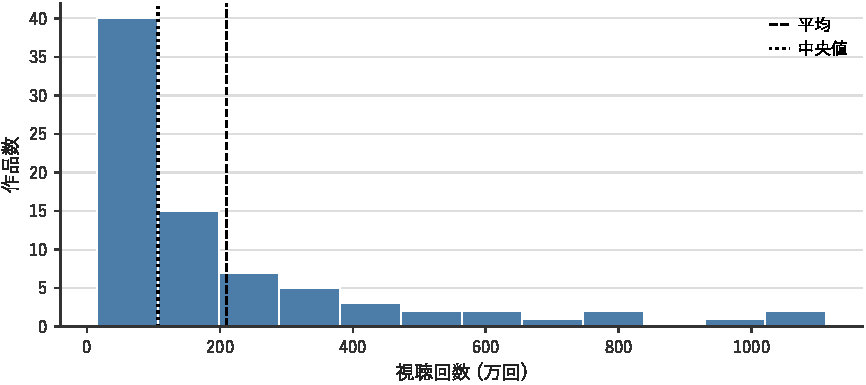
\includegraphics[width=0.85\linewidth]{../figures/output/ch02_views.pdf}
      \caption{映画80本の公開後30日間の視聴回数のヒストグラム. 横軸は視聴回数 (万回), 縦軸は作品の本数.}
      \label{fig:ch02-views}
    \end{figure}

    図を見ると, 左側の低い視聴回数のところに大きな山があり, そこから右側へ向かって細く長く裾が伸びている.
    大半の作品は左側の低い山に集まっていて, ごく一部の作品だけが右側の遠いところまで突き抜けている.
    平均の $209.4$ 万回という値は, この右に長く伸びた裾の大ヒット作に強く引っ張られて, 山の頂上よりもずいぶん右側にある.

  \subsection{手元にある分しか数えていない}

    この80本について計算した平均が $209.4$ 万回であることには, 何の疑いもない.
    80個の数値を電卓に入れて足し算し, 80で割れば, 誰が計算しても正確にこの数になる.

    しかし, この計算結果は「この動画配信サービスにある映画全般が, だいたいどれくらい見られているか」という疑問にまで答えてくれているだろうか.
    典型的な1本の姿を知りたいという問題なら, 平均ではなく中央値を見れば解決した.
    だが, この配信サービスで配信されている映画は, 全部で80本きりではないはずだ.
    手元にない残りの作品がどうなっているのかは, 手元にある80本をどう計算してもわからない.
    どの数を計算するかの問題ではなく, そもそも手元で数えた対象が「その80本」で途切れてしまっているからだ.

    最初に取り上げた商品のレビューを思い出してほしい.
    商品Bについていた20件のレビューは, その商品を買ったすべての人たちの声ではない.
    商品を買った人のうち, たまたまレビューを書き残してくれた20人分の記録にすぎないのだ.
    もし別の20人がレビューを書いていたとしたら, 平均が4.0になったとは限らない.
    評価が星5つであっても1人きりの意見なら信用しきれなかったのも, これと同じことだ.
    その1人がたまたま大満足した人だっただけで, 別の人なら星1つをつけていたかもしれないのである.

    映画の80本についてもまったく同じことが言える.
    いま手元にある80本の平均はたしかに $209.4$ 万回だった.
    しかし, もし別の80本を集めてきて同じように計算していたとしたら, この平均値は一体いくつになっていただろうか.

  \subsection{平均と期待値}

    ここで, 平均という計算と, 確率論で学んだ「期待値」とのつながりを整理しておこう.
    手元にある $n$ 個のデータからどれでも同じ確率で1つを選ぶとすれば, その選ばれた値の期待値は, データの平均とぴったり一致する.

    \begin{prop}{平均と期待値}{mean-expectation}
      重複を許して並べた $n$ 個の値 $x_1, x_2, \ldots, x_n$ からなる集まりから1つをランダムに取り出すとき, その値を確率変数 $X$ とする.
      このとき $X$ の期待値は
      \[
        E[X] = \frac{1}{n} \sum_{i=1}^{n} x_i = \bar{x}
      \]
      に等しい.
    \end{prop}

    詳しい証明は巻末の付録に譲る.

% 以下3つの図はコラム本体で参照するが, tcolorbox の中には float を置けないため, mybox の直前で宣言している.

% 図のデータ: 仮. 要作成
\begin{figure}[htbp]
  \centering
  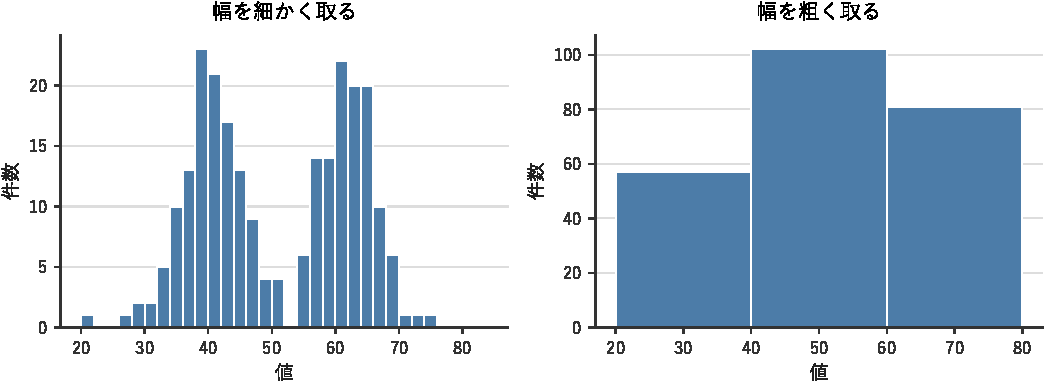
\includegraphics[width=\linewidth]{../figures/output/ch02_col_width.pdf}
  \caption{あるデータを二通りの階級の幅で描いたヒストグラム. 左は幅を細かく, 右は幅を粗く取っている.}
  \label{fig:ch02-col-width}
\end{figure}

% 図のデータ: 仮. 要作成
\begin{figure}[htbp]
  \centering
  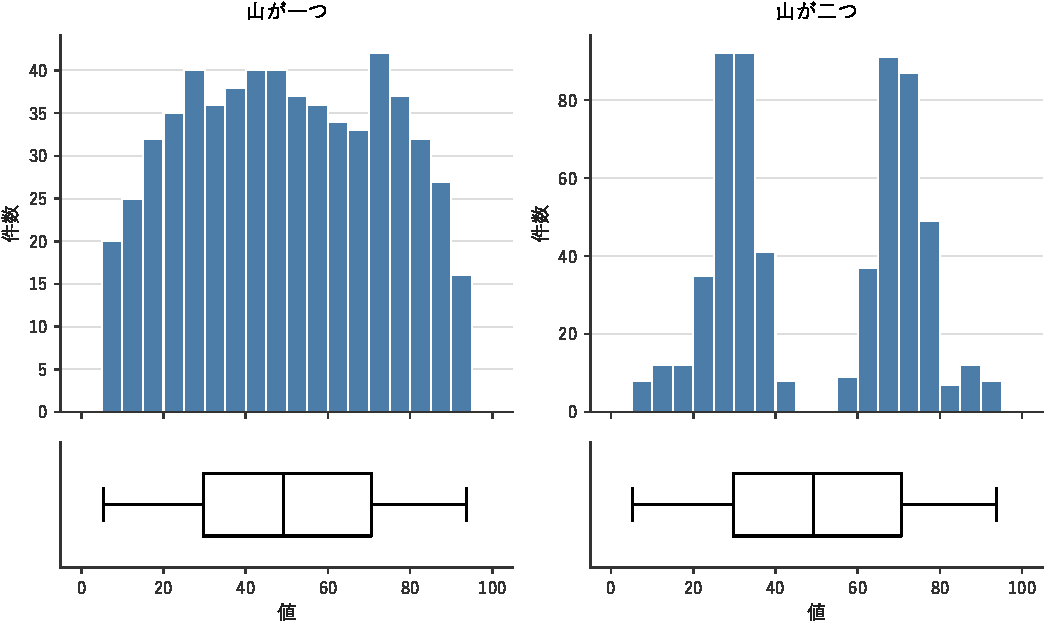
\includegraphics[width=\linewidth]{../figures/output/ch02_col_box.pdf}
  \caption{山が一つのデータと山が二つのデータを, ヒストグラム（上）と箱ひげ図（下）で描いたもの.}
  \label{fig:ch02-col-box}
\end{figure}

% 図のデータ: 仮. 要作成
\begin{figure}[htbp]
  \centering
  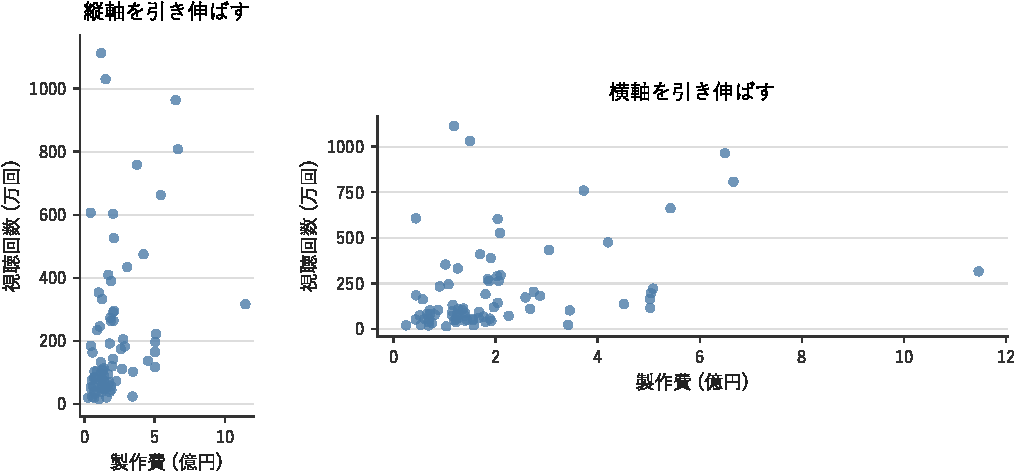
\includegraphics[width=\linewidth]{../figures/output/ch02_col_axis.pdf}
  \caption{同じ点を打った散布図を, 軸の縦横比だけ変えて並べたもの. 横軸は製作費 (億円), 縦軸は視聴回数 (万回).}
  \label{fig:ch02-col-axis}
\end{figure}

\begin{mybox}{数字を変えずに図を変える}

  \subsubsection*{階級の幅}

    ヒストグラムを描くときにデータをどのような幅で区切るかは, あらかじめ決まっているわけではなく, 描く人が自分で決めている.
    まったく同じ一つのデータを, 区切る幅を変えて二通りに描き分けてみたのが\cref{fig:ch02-col-width}だ.

    左側の細かく区切った図では山が二つ並んでいるように見えるが, 右側の粗く区切った図では一つのなだらかな山にまとまっている.
    元の数字は一つも変えていない. 変えたのは階級の幅だけだ.

    幅を細かくしすぎると, たまたま生じたわずかな偏りまでまるで意味のある山のように見えてしまう.
    逆に幅を粗くしすぎると, 全体の形は滑らかになるものの, 本当に二つに分かれていた特徴的な山まで一つにつぶれて見落とされてしまう.
    どちらか一方だけが絶対に正しい図だということはない.
    だからこそ, 一枚のヒストグラムだけを見て早合点してしまわないほうがよいのだ.
    いくつかの異なる幅で図を描いてみれば, どの幅でも共通して現れる特徴と, 区切り方によってたまたま現れた見かけの特徴とを見分けられるようになる.

  \subsubsection*{一番高い棒は何が多いのか}

    データの中で最も頻繁に現れる値には, 最頻値という名前がついている.

    \begin{defi}[unbreakable]{最頻値}{mode}
      観測値の中で最も頻繁に出現する値を\textbf{最頻値}と呼ぶ.
      最頻値は複数存在することもある.
    \end{defi}

    商品AやBのように点数そのものを数えた図であれば, 最も高い棒の点数がそのまま最頻値になる.
    商品Aなら4点, 商品Bなら5点だ.

    しかし, 映画の視聴回数のヒストグラムでは話が変わってくる.
    区間ごとにまとめて数えているため, 一番高い棒が示しているのは「その区間に入った映画の本数が最も多い」ということだけであって, その区間の中の具体的にどの値が一番多いのかまではわからない.
    しかも, 階級の区切り方を変えてしまえば, 最も高い棒が立つ位置そのものが左右に動いてしまうことすらある.

    なお, ヒストグラムの横軸は点数や視聴回数のように数字の大小順に並んでいるため, 棒の並び順を勝手に入れ替えることはできない.
    これに対して, 出身地や血液型のように順序のない項目を横軸に並べたものは棒グラフと呼ばれ, こちらは並び順を自由に入れ替えても図の意味は変わらない.
    見た目はよく似ていても, 横軸に並べているものが違う.

  \subsubsection*{五つの数に切り詰める}

    中央値は, データを小さい順に並べたときにちょうど真ん中に来る値だった.
    同じ考え方を使って, 真ん中以外の位置にある値を取り出すこともできる.

    \begin{defi}[unbreakable]{四分位数と四分位範囲}{iqr}
      観測値を小さい順に並べたとき, 下から $25\%$ の位置にある値を\textbf{第1四分位数} $Q_1$,
      下から $50\%$ の位置にある値を\textbf{第2四分位数} $Q_2$（中央値と一致する）,
      下から $75\%$ の位置にある値を\textbf{第3四分位数} $Q_3$ と呼ぶ.
      位置がちょうど何番目かに当たらないときは, 前後の観測値のあいだを, 位置の端数に応じて按分した値を使う.
      $Q_1, Q_2, Q_3$ をまとめて\textbf{四分位数}と呼ぶ.
      $Q_1$ と $Q_3$ の差
      \[
        \mathrm{IQR} = Q_3 - Q_1
      \]
      を\textbf{四分位範囲}（interquartile range）と呼ぶ.
    \end{defi}

    $Q_1$ から $Q_3$ までの区間には, データを順に並べたときの真ん中の $50\%$ 分のデータがすっぽり収まっている.
    四分位範囲は, その範囲の広さを表す数値だ.
    データの中央半分が狭い範囲に密集しているのか, それとも広く散らばっているのかを表している.

    この $Q_1$, $Q_2$, $Q_3$ と, データ全体の最小値と最大値を一つの図形にまとめたものが箱ひげ図だ.
    箱の中央に引かれた線が中央値で, 箱の両端が $Q_1$ と $Q_3$ を示し, 箱の長さが四分位範囲を表す.
    そして箱の両端から伸びるひげの端点が, 一番小さい値と一番大きい値を表している.

    箱ひげ図を使うとデータ全体がコンパクトな記号にまとまるため, たくさんのグループを横に並べて比較するときに重宝する.
    たとえば映画をジャンルごとに分けて並べれば, それぞれの中央値の高さや散らばりの大きさを一目で比べることができる.
    ヒストグラムを何枚も並べて見比べるよりもはるかに手軽だ.

    ただし, 箱ひげ図は中央値, $Q_1$, $Q_3$, そして両端の最小値と最大値という, たった五つの数だけを使って描かれていることには注意がいる.
    \cref{fig:ch02-col-box}を見てほしい.
    ヒストグラムで見れば一方は山が一つ, もう一方は山が二つに割れていて明らかに形が違うのに, 箱ひげ図にしてしまうとどちらもほぼ同じ形になってしまう.
    箱の中央に線があるからといって, そこにデータが一番たくさん集まっているとは限らないのだ.

    五つの数しか使っていないからこそ並べて比べやすいのだが, 逆に五つの数しか使っていないからこそ, データの重要な山や谷の形が消えてしまうのである.

  \subsubsection*{軸を引き伸ばす}

    二つの数量の関係を調べたいときは, データを1点ずつ平面に打っていく.
    横軸に製作費, 縦軸に視聴回数を取れば, 1本の映画は座標平面上の1個の点になる.
    こうしてすべての映画を点で打った図を散布図と呼ぶ.

    \cref{fig:ch02-col-axis}にある二枚の散布図は, まったく同じデータを打ったものだが, グラフの縦横の比率だけを変えてある.
    縦軸を引き伸ばすとデータは急勾配の右上がりに見え, 逆に横軸を引き伸ばすとごく緩やかな傾きに見える.

    階級の幅を変えたときは, 少なくともまとめ方の数え直しは行っていた.
    だが散布図の縦横比を変えるときは, 数え直しすらしていない. 製作費と視聴回数の数字は少しも動かしていないのだ.
    それでも, 目から入ってくる印象はまるで違ったものになってしまう.

  \subsubsection*{描く前に決まっていること}

    数字は一つも書き換えていないのに, 図のまとめ方を変えるだけで見えるものが何度も入れ替わった.
    区切りの幅, 一番高い棒の意味, 五つの数への切り詰め, そしてグラフの縦横比.
    元データそのものは何も変わっていないのに, 図の上ではまったく違う印象が現れてくる.

    図というのは, データをありのままに写し取ったものではない.
    どこで区切り, どの比率で軸を取るかという判断が入って, はじめて一枚の図になる.
    そしてこれは, 統計量という数についても同じことだ.
    何を知るために計算するのかをあらかじめ決めてはじめて, その数で何が言えるのかが決まる.
    決めるのは, データではなく, 自分が何を知りたいかのほうだ.
\end{mybox}


\newpage

% 第3章 = 第2段「一つの数も, 取り直せば散らばる」
\section{一部と全部：分布と中心極限定理}

  \subsection{毎回変わってしまう待ち時間}

    話題のラーメン屋さんに行ってみると行列ができている.
    あなたは今このくらいの人数並んでいるからおおよそこのくらいの時間で自分の順番がくるだろうと考えて並ぶ.
    しかし, 実際のところその予想は当たらないことが大半だろう.
    すぐに行列が消化されてラッキーと思うこともあれば, 全然進まず別の店に行くか迷うこともある.
    とはいえ, 30人くらい並んでいたとしたら, 「絶対1時間以上待つだろう」と明らかにわかることもある.
    より正確に, それぞれの待ち時間がどのくらいの確率で起きるかを見積もるには, 人数や時間帯, 曜日などを加味してどのくらい待つものなのかたくさん経験してみるしかない.
    そうすると, 完全に正確な待ち時間をぴたりと当てることは難しいにせよ, おおまかな傾向はつかめるはずだ.
    このとき, 我々は「データの分布」というものを無意識のうちに考えている.
    たとえば100回通って取った待ち時間の記録がどのように分布しているかを確認することによって,
    その背後にある, 全ての記録を含むような神様しか知らない「本当の分布」から計算される, それぞれの待ち時間がどのくらいの確率で起きるかを見積もっているのだ.

  \subsection{手元のデータとその出どころ}

    ラーメン屋に100回通って取った記録から平均を出したとしても, 別の100回ならその平均も少し違う数になるだろう.
    前の章の終わりに残った, 映画80本の疑問もこれと同じだ.
    手元の80本を平均すれば $209.4$ 万回になることは間違いないが, 別の80本でもそうなるとは限らない.
    大ヒット作が多めに入って $230$ 万回になるかもしれないし, そうした作品が少なくて $190$ 万回に下がるかもしれない.
    計算を何度やり直しても答えは同じなのに, 計算する相手を取り直すと答えが変わってしまうのである.

    この手元にある分と, その背後にある全部とを区別するために, 名前をつけておこう.

    \begin{defi}{母集団と標本}{population-sample}
      調査や分析の対象となる集まり全体を\textbf{母集団}と呼ぶ.
      その母集団から実際に観測するために取り出された一部のデータを\textbf{標本}と呼び,
      標本に含まれるデータの個数を\textbf{標本サイズ}と呼ぶ.
    \end{defi}

    映画なら, その配信サービスで配信されている対象作品全体が母集団で, 手元の80本が標本になる.
    標本サイズは $n = 80$ だ.
    本当は全部の様子を知りたいのだが, 全部を調べるのは難しいので, 一部を使って見当をつけようとしている.
    待ち時間の記録から本当の分布を考えたのと, やっていることは同じである.

    ただ, 一部なら何でもよいというわけにはいかない.
    ランキング上位の人気作ばかり80本集めてきたら, 平均が高くなるのは当たり前だろう.
    足し算も割り算も正しくできているのに, 作品全体の様子からは離れてしまう.
    我々は計算を始める前に, すでに大事なことを決めてしまっているのだ.
    以下では, この80本は対象作品全体から大きな偏りなく選ばれた標本として扱うことにする.

  \subsection{偏ったサイコロの平均}

    さて, 取り直せば平均が変わることはわかったが, どれくらい変わるものなのだろうか.
    元のデータが極端に偏っていれば, 平均の分布も同じように偏りそうな気がする.
    そもそもそのデータを足して割っただけなのだから, そう思うのも無理はない.
    サイコロで試してみよう.

    使うのは, 1の目が出る確率が $50\%$ で, 2から6の目はそれぞれ $10\%$ ずつしか出ないサイコロだ.
    ふつうのサイコロならどの目も同じ確率で出て, 理論上の平均は3.5になる.
    こちらは1が半分を占めるので, 理論上の平均は2.5だ.
    出目の確率を棒で描くと, 1のところだけが高く, あとは平らに並ぶ形になる.
    これがこのサイコロの本当の分布である.
    ラーメン屋の待ち時間と違って, 今回は我々が確率を決めたので, 神様の側から先に形を知っているわけだ.

    このサイコロを5回振り, 出た目を足して5で割る.
    それだけでは平均は一つしか出てこないので, 「5回振って平均を出す」ところまでを1000回繰り返してみる.
    こうして集まった1000個の平均を, ヒストグラムにする.
    さらに, 5回を30回に増やして同じことをやってみたのが\cref{fig:ch03-dice-clt}だ.

    \begin{figure}[htbp]
      \centering
      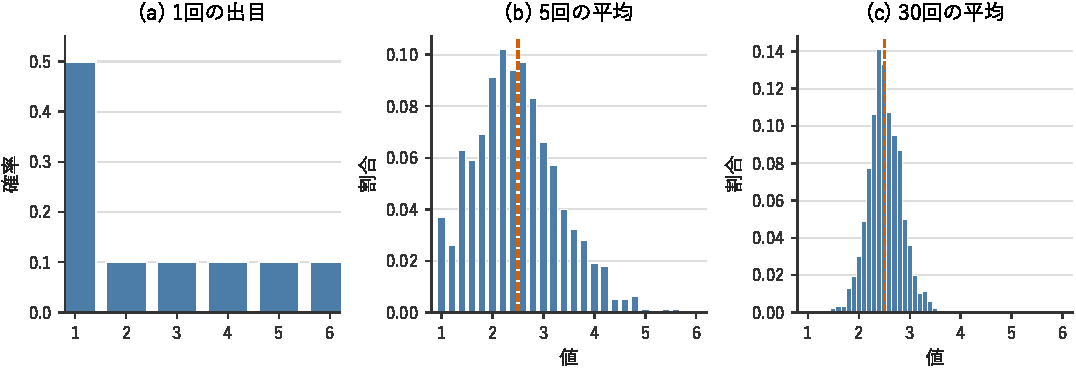
\includegraphics[width=\linewidth]{../figures/output/ch04_dice_clt.pdf}
      \caption{偏ったサイコロの出目と標本平均の分布. 破線は理論上の平均2.5. 5回または30回振って平均を取る操作を1000回ずつ繰り返した. 5回の平均は0.2刻みの値しか取らないため, (b)の棒は櫛状に並ぶ.}
      \label{fig:ch03-dice-clt}
    \end{figure}

    (a)では1の棒だけが高かったのに, 5回の平均を集めた(b)には, まだ少し左に偏っているものの, なだらかな山が現れている.
    30回の平均を集めた(c)では, 2.5を中心にした左右対称の釣鐘型にかなり近くなった.
    サイコロをまともなものに取り替えたわけではない.
    相変わらず半分は1が出るサイコロを振っているのに, 30個を足して割るだけで, 平均の分布は元の出目と似ても似つかない形になっている.
    平均を取るというのは, ずいぶん面白いことをしていたのである.

  \subsection{標本分布と中心極限定理}

    今の実験では, 振るたびに出てくる目を数える代わりに, 何回か振るたびに出てくる平均を数えた.
    前の章でたくさんの値を一つにまとめたばかりなのに, その一つの数も集め直せばまたたくさんになって, 分布が描ける.
    この分布にも名前がついている.

    \begin{defi}{標本分布}{sampling-dist}
      母集団から標本を繰り返し取り直し, そのたびに統計量を計算するとき, その統計量の値が従う確率分布を, その統計量の\textbf{標本分布}と呼ぶ.
    \end{defi}

    名前に「標本」と入っているが, 標本分布は手元にあるデータそのものの分布ではない.
    サイコロの図の(a)は, 振る前から決まっている出目の本当の分布だった.
    (b)と(c)は, 標本を取り直しては平均を計算することを繰り返して描いた, 平均の標本分布の様子なのである.

    サイコロの平均が釣鐘型に近づいたのは, たまたまうまい具合に目が出たからではない.
    振る回数を増やすとどうなるかについて, 次のことがわかっている.

    \begin{thm}{中心極限定理}{clt}
      平均 $\mu$, 分散 $\sigma^2$ をもつ同一の分布から, 互いに独立に $n$ 個の値を取り出し, その標本平均を $\bar{X}$ とする.
      $n$ が大きくなるにつれて, $\bar{X}$ の標本分布は正規分布 $N\!\left(\mu,\; \sigma^2 / n\right)$ に近づく.
    \end{thm}

    同じ分布から互いに独立に値を取り出すことを, \textbf{独立同分布}という.
    サイコロなら, 毎回同じサイコロを, 前の出目とは関係なく振るということだ.
    この条件のもとでは, 元の分布が釣鐘型でなくてもよい.
    段差のあるサイコロでも, 右に裾を引く映画の視聴回数でも, 平均を作る個数 $n$ を増やせば, 平均の分布は釣鐘型に近づいていく.
    「$n$ が大きくなるにつれて」とあるのは, 少ない個数でもぴったり同じ形になると言っているわけではないからだ.
    どのくらいの速さで近づくかは, 元の分布によって違う.

    この釣鐘型が\textbf{正規分布}で, 中心の平均値 $\mu$ と, 散らばりの大きさを表す標準偏差で形が決まる.
    平均値から左右に標準偏差2つ分の範囲を取ると, 全体の約 $95\%$ が入るという性質がある.
    形がわかるというのは, どこにどれくらい集まるかまでわかるということなのだ.

    さらに定理の式には, サイコロの図でも見えていたことがもう一つ書かれている.
    平均の分布の分散は, 元の値の分散 $\sigma^2$ を $n$ で割った $\sigma^2/n$ になる.
    個数を増やすと釣鐘型に近づくだけでなく, 中心の $\mu$ のまわりに狭く集まってくるのである.

    \begin{mybox}{分布という言葉について}
      前の章では, データがどのあたりに多く集まり, どこに少ないかという全体の姿を「分布」と呼んだ.
      ところが今は, 振る前のサイコロにも, 取り直した平均にも同じ言葉を使っている.
      手元のデータの話だったはずなのに, いつの間にか話が広がっているではないか.
      「分布」は形を指す言葉で, 何の形なのかは, 何を数えているかで決まるのである.

      映画80本のヒストグラムは, 視聴回数の区間ごとに作品を数えた記録の分布で, 前の章の意味そのままだ.
      サイコロの図の(a)は, どの目がどの確率で出るかという本当の分布である.
      1が $50\%$ という決まりは振る前からあり, 手元に記録があってもなくても変わらない.
      そして(b)(c)で数えたのは, 取り直すたびに計算した平均だ.
      どれも棒の絵で描けるが, 記録, 本当の分布, 統計量の分布, つまり本文で標本分布と呼んだものと, 描いているものが違っている.

      まず, 記録は本当の分布から得た一部分で, 偏りなく記録を増やせば, ヒストグラムの形は本当の分布に近づいていく.
      だから手元の80本を, 全体の代役にしてみることもできるわけだ.
      次に, 統計量の分布は, 本当の分布と標本サイズ $n$, それにどんな計算をするかで決まる.
      サイコロの(a)から30回分を取って平均を作ると(c)になる, というのがその実例である.

      では, 正規分布という釣鐘型はどこに出てくるのだろうか.
      これは形につけた名前なので, 三つのどこに現れてもよい.
      同じ分布から独立に取った値を足すと釣鐘型に近づく, というのが中心極限定理の言っていることで, 平均も足し算をしているから釣鐘型に近づく.
      身長のように, 同じ分布とは限らない多くの要因が足し合わさったものにも似た性質が知られていて, 身長の形が釣鐘型に近いのはそのためだと説明される.
      ただし, この本では, データそのものが正規分布だとは仮定しない.
      正規分布を使うのは, 平均やその差といった統計量が, 取り直したときにどんな分布になるかを考える場面だけだ.

      本当の分布は, 調べる相手によって形が違う.
      ふつうのサイコロならどの目も同じ確率の一様分布, 同じ確率で独立に当たり外れを繰り返したときの当たりの回数なら二項分布が出てくる.
      めったに起きないことの回数にはポアソン分布, 測定値などには釣鐘型の正規分布が使われることもある.
      もっとも, 映画の本当の分布はこのどれでもなく, 右に裾を引いた形だ. 本当の分布に名前があるとは限らないのである.

      一方, 本当の分布がどんな形でも, 平均は $n$ を大きくすると正規分布に近づく.
      正規分布から取ったデータなら, 平均が本当の平均からどれだけずれているかを, 分からない $\sigma$ の代わりに手元のデータから計算した標準偏差を使って測ると, その数は正規分布ではなく $t$ 分布という親戚に従う.
      $n$ が大きければ正規分布と見分けがつかない. 後の章の検定で名前が出てくる.
      同じく正規分布から取ったデータなら, 手元のデータから計算した分散がどんな分布になるかも分かっていて, 尺度を除けばカイ二乗分布と呼ばれる形になる. これも正規分布から作られた親戚である.
      独立に見積もった二つの分散の比を扱う親戚には $F$ 分布もあるが, カイ二乗分布と $F$ 分布はこの本の本文では使わない.

      正規分布が本当の分布と統計量の分布の両方に現れる理由は, 足し算にある.
      二項分布が試行回数 $n$ を増やすと正規分布に近づくのも, 当たりか外れかを足しているからで, その平均に中心極限定理を当てたのと同じことだ.
      本当の分布の形はいろいろだが, この本で扱う統計量の形は, 正規分布とそこから作られた親戚でほとんど足りる.
      この本で先に出てくる分布の名前はこれで全部である.
    \end{mybox}

  \subsection{平均のばらつきを計算する}

    分散が $\sigma^2/n$ なら, 平方根を取った標準偏差は $\sigma/\sqrt{n}$ だ.
    これが, 取り直したときに平均がどれくらい動くかを表す数になる.
    平均を何度も取り直して並べなくても, 元の値の標準偏差と個数から計算できてしまう.

    \begin{defi}{標準誤差}{se}
      母集団の標準偏差を $\sigma$, 標本サイズを $n$ とするとき, 標本平均の\textbf{標準誤差}（SE: Standard Error）を
      \[
        \mathrm{SE} = \frac{\sigma}{\sqrt{n}}
      \]
      と定義する.
    \end{defi}

    とはいえ, このままでは少し困る.
    分子の $\sigma$ は本当の分布の標準偏差なのに, 我々はその全部を調べられないから一部を使っていたのだった.
    そこで, 手元の標本から計算した標準偏差に代役を頼むことにする.

    ただし, 前の章で使った分散 $s^2$ をそのまま使うのではなく, 割る数を $n$ から $n-1$ に変える.

    \[
      u^2 = \frac{1}{n-1}\sum_{i=1}^{n}(x_i-\bar{x})^2, \qquad u = \sqrt{u^2}
    \]

    この $u^2$ を\textbf{不偏分散}といい, その平方根 $u$ で本当の標準偏差を見積もる.
    手元のデータ自身をまとめるときと, その背後にある全部のばらつきを見積もるときとで, 割る数が少し違うのである.
    なぜそうするのかはこの節の終わりのコラムに譲って, 今はこの $u$ を使って計算を進めよう.
    実際に手元で計算する標準誤差は,
    \[
      \mathrm{SE} = \frac{u}{\sqrt{n}}
    \]
    となる.

    標準偏差と標準誤差は名前がよく似ているので, どちらも同じようなものに思えるかもしれない.
    しかし $u$ が見ているのは一本一本の映画の違いで, 標準誤差が見ているのは, 映画を選び直すたびに出てくる平均の違いだ.
    本数を増やしたからといって, 大ヒット作とほとんど見られない作品との差が縮まるわけではない.
    だから個々の値のばらつきを見積もる $u$ は, データを増やしてもそれだけで小さくはならない.
    一方, 標準誤差には分母に $\sqrt{n}$ があるので, 本数を増やすと小さくなる.
    一本一本の違いは大きいままでも, まとめて平均を取ると, 取り直しによる違いを小さくできるのである.

    \begin{mybox}{なぜ $n-1$ で割るのか}
      分散を計算するとき, データの記述では個数 $n$ で割っていたのに, 母集団の分散を見積もるときには $n-1$ で割った.
      この「1を引く」ことにはどんな意味があるのだろうか.

      手元にあるデータから分散を計算するとき, 本当なら母集団全体の真の平均 $\mu$ からのずれを測りたい.
      ところが $\mu$ は分からないので, 代わりに手元の標本平均 $\bar{x}$ を使って $(x_i - \bar{x})^2$ を計算する.

      $\bar{x}$ は, 手元にあるデータのちょうど真ん中に来るように作った値だ.
      データ自身の平均からのずれを二乗して足し合わせると, ほかのどんな基準値を使ったときよりも合計が小さくなってしまう性質がある.
      真の平均 $\mu$ は手元の $\bar{x}$ と少しずれた場所にあるはずなので, $\bar{x}$ から測った二乗の合計は, $\mu$ から測ったときより小さめに出てしまう.

      その分を補正するために, 分母の $n$ を少し小さくして $n-1$ で割っている.
      手元のデータ数が80件なら, $n$ で割るのと $n-1$ で割るのとで結果の差はごくわずかだが, 理屈の上ではこのような差の調整が行われている.
    \end{mybox}

  \subsection{映画の平均はどれくらい動くか}

    それでは, 映画でもサイコロと同じことが起きるのか, 試してみよう.
    対象作品全体から80本を何度も取り直せればよいのだが, 手元にあるのは今の80本だけだ.
    ひとまずこれを全体の代役にして, その中からランダムに20本を選んで平均を出すことにする.
    一度選んだ作品は候補に戻してから次の1本を選ぶ. これを復元抽出という.
    同じ作品がまた選ばれることもあるが, こうしておけば, 前に何を選んだかで次の候補が変わらずにすむ.
    「20本を選んで平均を出す」ところまでを1000回繰り返して, 1000個の平均を並べてみる.

    もちろん, この実験で選べるのは, あくまで手元にある作品だけである.
    全体から取り直すことを完全に再現しているわけではないが, 平均がどう動くかの見当はつけられる.

    \begin{figure}[htbp]
      \centering
      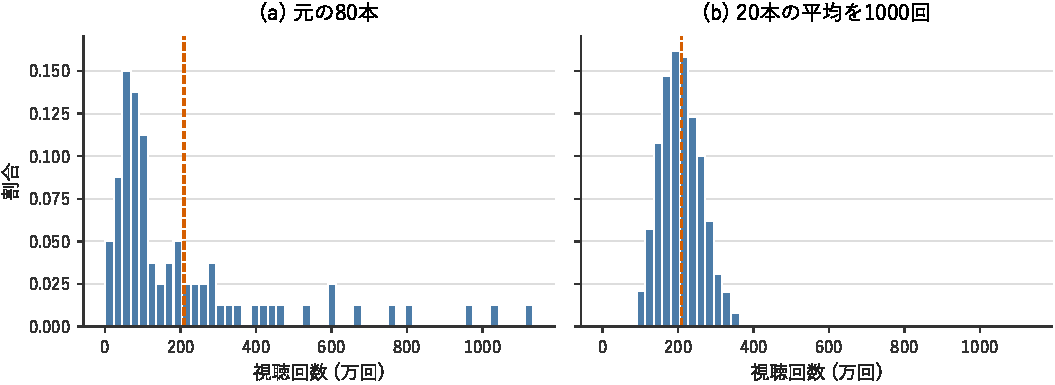
\includegraphics[width=\linewidth]{../figures/output/ch04_sampling_dist.pdf}
      \caption{元の映画80本の視聴回数と, 80本から20本を復元抽出して求めた標本平均の分布. 復元抽出と平均の計算を1000回繰り返した. 横軸と縦軸の尺度は左右で共通で, 破線は80本全体の平均を示す.}
      \label{fig:ch03-sampling-dist}
    \end{figure}

    \cref{fig:ch03-sampling-dist}の左は, 元の80本の視聴回数だ.
    右に長い裾を引いていた形が, 20本ずつの平均を1000回集めた右の図では, 左右対称の釣鐘型にかなり近くなっている.
    選べる作品は左の図にあるものだけなのに, 平均を計算して並べると, こんなに違う姿になるのだ.
    左右で横軸の目盛りをそろえてあるので, 平均の散らばる幅がずっと狭くなっていることもわかる.

    さて, 今の実験は20本の平均だったが, 知りたかったのは80本の平均 $209.4$ 万回がどれくらい動くかだった.
    もう一度実験をしなくても, 今度は標準誤差の式で計算できる.
    標本サイズは $n = 80$ で, $n-1 = 79$ で割って求めた標準偏差 $u$ はおよそ $240.8$ 万回になる.
    前の章で $n = 80$ で割って求めた $s$ は $239.3$ 万回だったので, 少しだけ大きくなった.
    $\sqrt{80} \approx 8.94$ を使うと,

    \[
      \mathrm{SE} = \frac{u}{\sqrt{80}} \approx \frac{240.8}{8.94} \approx 26.9
    \]

    となり, 標準誤差はおよそ $26.9$ 万回だ.
    先ほどの20本から80本へと本数が4倍になると, 分母は $\sqrt{4} = 2$ 倍になる.
    つまり, 平均のばらつきは20本のときの半分ほどになる計算だ.
    本数を増やすのは大変なのに, ばらつきが小さくなるのは, その平方根の分だけなのである.

    一本一本の映画は, 何百万回も見られる作品からほとんど見られない作品まであって, 標準偏差でいえば $240$ 万回も散らばっていた.
    それが80本の平均になると, 別の80本を取り直したときのばらつきは, 標準誤差でおよそ $27$ 万回になる.
    最初の $209.4$ 万回という数だけではわからなかった, 取り直すとどれくらい動くかという大きさまで, 手元の80本だけから計算できたのである.

  \begin{mybox}{ここまででわかったこと}
    四段階の三つ目「ばらつきを見積もる」.

    \textbf{この章で言えるようになったこと}: 一本一本の映画は標準偏差で約 $240$ 万回も散らばるが, 80本の平均を取り直したときのばらつきは, 標準誤差で約 $27$ 万回と見積もれた.
    対象作品全体から大きな偏りなく選ばれた標本として扱えば, 手元の80本だけからこれを計算できる.

    \textbf{まだ言えないこと}: 取り直した平均がどれくらい動くかはわかったが, 作品全体の本当の平均はどのあたりにあるのだろうか.

    \textbf{前の章の見方がどう変わったか}: 手元の80本が決まれば, 平均は $209.4$ 万回に決まる.
    だが, 別の80本を集めれば, その一つの数も変わる.
  \end{mybox}


\newpage

% 第4章 = 第3段「今回の答えが当たったかは分からなくても, その作り方がどれだけ当たるかは言える」
\section{全体の平均を見積もる：統計的推定}

  \subsection{スープの味見をする}

    家でカレーや鍋, スープを作っているとき, おおよそできたかなというタイミングでスプーンで一口味見をする.
    この味見はどれくらいスープ全体の味を反映しているだろうか.
    それは十分混ぜたし, だいたいランダムに掬う場所を決めたのだから, おおよそ全体の味がそのまま一口に凝縮されているはずだ.
    しかしこれが例えば, 醤油を足してすぐ, その足した場所付近を取ってきてしまったら, ほとんど醤油の味しかしないだろう.
    私たちはこのように割と自然に, 味見の結果がもっともらしいものになるようにうまく調整している.
    手元のデータも全体の情報をきちんと反映している, もっともらしいものであってほしい.
    とはいえ, スープのようにデータがもっともらしいものになるように調整して取ってくるのは至難の業である.
    そこで, 手元のデータについて, どのくらいばらつきがありそうか, を計算して全体の様子をばらつき分の余裕をもって推定することにしよう.
    これが区間推定と呼ばれるものの考え方である. 

  \subsection{母平均はどこにいるのか}

    前の章で, 映画80本の平均視聴回数から標準誤差を計算した.
    手元の平均は $209.4$ 万回で, 標準誤差はおよそ $26.9$ 万回だった.

    しかし, 本当に知りたかったのは, 手元の80本の平均そのものというより, その背後にある作品全体の平均のはずだ.
    この母集団全体の平均を\textbf{母平均}と呼ぶ.
    母平均は, 調査する前からどこかに決まっていて動かない値だが, その値は分からない.

    手元にある $209.4$ 万回という数字を, そのまま「母平均だ」と言い切ってしまうのは心もとない.
    前章で確認したように, 別の80本を集め直せば平均は少し違う値になってしまうからだ.

    ただ, 平均がどれくらい動くかであれば, 標準誤差としてすでに計算できている.
    動く大きさの見当がついているのなら, そのぶんだけ余裕を持たせて, 「母平均はだいたいこのあたりからこのあたりまでにいそうだ」という範囲でなら言えそうだ.

    小さな例で考えてみよう.
    ある商品のレビューが全体で1000件あり, 手元にはそのうち50件だけがあるとする.
    50件の平均は $\bar{x} = 4.2$, 標準偏差は $u = 0.7$ だったとしよう.
    標準誤差を計算すると, $\mathrm{SE} = 0.7 / \sqrt{50} \approx 0.10$ になる.

    ここで中心極限定理を思い出すと, 標本サイズがそこそこ大きければ, 標本平均はおよそ正規分布に従うのだった.
    その正規分布の標準偏差が標準誤差なので, 標本平均は中心の $\mu$ から左右に標準誤差の2倍, より正確には $1.96$ 倍の範囲に, およそ $95\%$ の確率で収まる.

    ただし, 手元にあるのは $\mu$ ではなく標本平均のほうだ.
    標本平均が $\mu$ からある距離の内側にあるなら, $\mu$ も標本平均から同じ距離の内側にある.
    そこで, 手元の標本平均を中心に, 左右へ $1.96 \times \mathrm{SE}$ ずつ広げた範囲を作る.

    \begin{defi}{95\%信頼区間}{ci95}
      標本平均を $\bar{x}$, その標準誤差を $\mathrm{SE}$ とするとき,
      \[
        \bar{x} - 1.96 \times \mathrm{SE} \;\leq\; \mu \;\leq\; \bar{x} + 1.96 \times \mathrm{SE}
      \]
      を満たす範囲を, 母平均 $\mu$ の\textbf{95\%信頼区間}と呼ぶ.
    \end{defi}

    手元の計算では, $1.96$ を「およそ2」と丸めて $\bar{x} \pm 2 \times \mathrm{SE}$ と計算して差し支えない.
    先ほどのレビュー50件の例でいえば, $4.2 \pm 2 \times 0.10$, つまり $4.0$ から $4.4$ という範囲になる.
    前章で計算した「平均がどれだけ動くか」という標準誤差が, ここで「母平均がどこからどこまでにいそうか」という範囲に姿を変えた.

  \subsection{区間の信用はどこにあるのか}

    こうして $4.0$ から $4.4$ という区間が手に入った.
    では, この「95\%」という数字は何を意味しているのだろうか.
    「母平均が95\%の確率でこの区間に入っている」と言いたくなるかもしれないが, それは少し違う.

    母平均 $\mu$ は, 誰にも分からないが, すでに決まった一つの値であって動かない.
    動くのは手元のデータから計算した標本平均 $\bar{x}$ のほうであり, それに伴って区間の位置も動く.

    この仕組みは, 母平均をあらかじめ知っている視点から眺めてみるとはっきりする.
    レビュー全体の平均が $\mu = 4.1$, 標準偏差が $0.7$ だと分かっている母集団から, 50件の標本を取り出して $\bar{x} \pm 2 \times \mathrm{SE}$ の区間を作る.
    この作業を100回繰り返したシミュレーションが, \cref{fig:ch04-ci-coverage}だ.

    \begin{figure}[htbp]
      \centering
      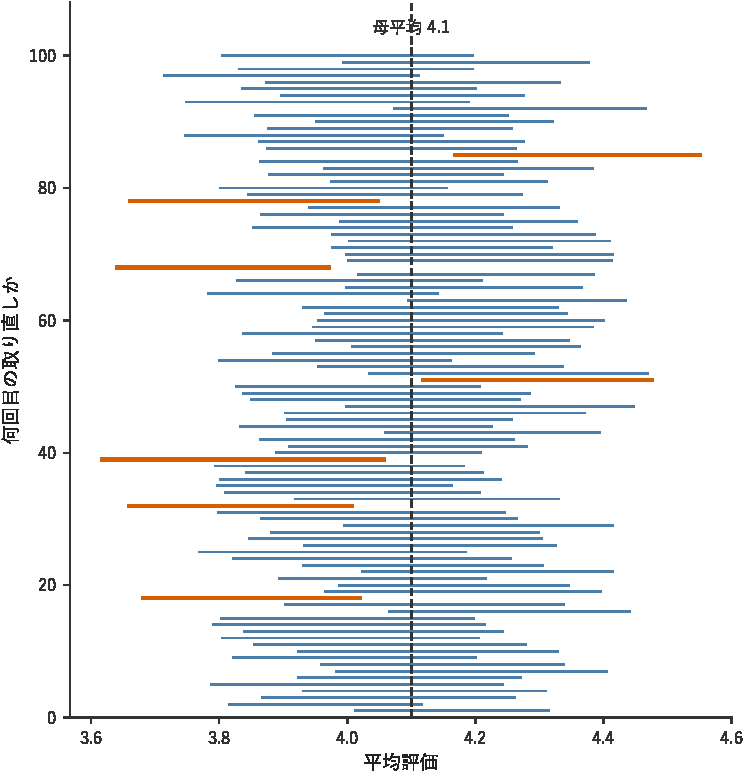
\includegraphics[width=0.8\linewidth]{../figures/output/ch05_ci_coverage.pdf}
      \caption{母平均4.1, 標準偏差0.7の母集団から50件の標本を取り, 95\%信頼区間を作る手順を100回繰り返した結果. 横棒の1本1本が1回分の区間を示す. 縦の破線は母平均4.1で, 動かない. 100本のうち93本(細い棒)は母平均を含み, 7本(太い棒)は外している.}
      \label{fig:ch04-ci-coverage}
    \end{figure}

    図を見ると, 100本の区間のうち93本は母平均の破線を含んでいるが, 7本は外してしまっている.
    きっかり95本にならないのは偶然で, この100回を別の機会にやり直せば, 含まれる本数は95本の前後に散らばる.

    図の棒は, どの1本も, 母平均を含んでいるか, 含んでいないかのどちらかで, 「95\%の確率で含んでいる」棒は1本もない.
    手元で作った $4.0$ から $4.4$ という区間も, 当たりか外れかのどちらかだ.
    ただ, 母平均を知らないかぎり, どちらなのかを確かめるすべはない.

    それなら, 手元の一本の区間など頼りにならないのではないか, と思えるかもしれない.
    それでもこの区間を信頼して使えるのは, 区間そのものが絶対だからではなく, 区間を作った手順のほうを信じているからだ.
    だから「95\%信頼区間」の95\%は, この区間に $\mu$ がある確率ではなく, 同じ手順で作った区間には, 100回に95回ほど母平均が入る, という意味だ.

  \subsection{区間があると何が変わるか}

    新しい薬の治験を行って, 「血圧を平均で 5\,mmHg 下げた」という結果が得られたとする.
    もしこの結果の95\%信頼区間が 2\,mmHg から 8\,mmHg だったとすれば, 取り直しのばらつきを考慮しても, おそらく少なくとも 2\,mmHg くらいは下がりそうだと見当がつく.
    医師もこれなら投薬の判断がしやすい.

    ところが, 同じ「平均 5\,mmHg 下がった」という結果であっても, 95\%信頼区間を計算してみたら $-1$\,mmHg から 11\,mmHg だったとしたらどうだろうか.
    区間の中にゼロやマイナスが含まれているということは, 本当の効果がまったくないことも, むしろ血圧が上がることも, 今回のデータからは否定できないということだ.
    そうなると, 軽々しく薬を使うわけにはいかなくなる.

    手元の標本平均が「5」であることだけを見ていたら, この二つの状況の違いには気づけない.
    幅があれば, 見積もりの値だけでなくその精度までわかるから, 過大な評価をうのみにしたり, 判断を誤ったりせずにすむ.

    区間の広さを決める手続きのうち, 何が数理的な必然で, 何が人間の選択なのかも整理しておこう.
    標本平均の分布が正規分布に近づくという事実は, 中心極限定理が保証するもので, 人間の都合で変えることはできない.
    一方で, 「100回に何回母平均が入るように作るか」という割合は, 計算する人間が目的に応じて選ぶものだ.
    この割合を\textbf{信頼水準}と呼ぶ.

    信頼水準を変えれば, 標準誤差に掛ける数字が変わる.
    \begin{itemize}
      \item 90\%なら $\pm 1.64 \times \mathrm{SE}$
      \item 95\%なら $\pm 1.96 \times \mathrm{SE}$
      \item 99\%なら $\pm 2.58 \times \mathrm{SE}$
    \end{itemize}

    99\%に設定すれば, 母平均を外してしまう区間は100回に1回ほどに減らせるが, そのかわり区間は左右に大きく広がってしまう.
    逆に90\%にすれば区間を狭く絞り込めるが, 10回に1回くらいは母平均を逃す区間ができるのを受け入れなければならない.
    世の中で95\%がよく使われるのは, 狭さと外しにくさの折り合いがほどよくつくという実用上の都合であって, 何か特別な理論的根拠があるわけではない.

    なお, 標本サイズが小さいときには, この「およそ2」という倍率をもう少し大きめに見積もる必要がある.
    本書では, 標本サイズがそこそこ大きくて倍率が2のままで足りる場合を考えていく.

  \subsection{映画の視聴回数を見積もる}

    映画80本のデータに戻ってみよう.
    手元の平均 $209.4$ 万回と標準誤差 $26.9$ 万回を使って, 95\%信頼区間を計算してみる.
    中心の $209.4$ から左右に $2 \times 26.9 = 53.8$ 万回だけ広げればよい.

    \[
      209.4 \pm 2 \times 26.9 \;\Rightarrow\; 155.6\;\text{万回} \;\sim\; 263.2\;\text{万回}
    \]

    およそ 156 万回から 263 万回という区間が得られた.
    手元の80本だけを計算した平均は確かに 209 万回だったが, 作品全体の本当の平均がそこからどれくらい外れうるかは, この区間を見ることで初めて見当がつく.

  \subsection{件数が増えると何が起きるか}

    前々章で, 星5つのレビューがついている商品があっても, レビューを書いたのがたったの1人だけなら素直に信じる気にはなれない, という話をした.
    その不安の正体も, 区間の広さとして捉え直すことができる.

    同じ平均 $3.8$, 標準偏差 $u = 0.9$ を示す商品であっても, レビューの件数 $n$ が異なると区間がどうなるかを見てみよう.
    \begin{itemize}
      \item $n = 5$ のとき: $\mathrm{SE} = 0.9 / \sqrt{5} \approx 0.40$ より, 区間は $3.8 \pm 0.80$ (3.0 〜 4.6)
      \item $n = 20$ のとき: $\mathrm{SE} = 0.9 / \sqrt{20} \approx 0.20$ より, 区間は $3.8 \pm 0.40$ (3.4 〜 4.2)
      \item $n = 100$ のとき: $\mathrm{SE} = 0.9 / \sqrt{100} = 0.09$ より, 区間は $3.8 \pm 0.18$ (3.62 〜 3.98)
    \end{itemize}

    手元の平均はどれも同じ $3.8$ だ.
    しかし, $n = 5$ のときの区間は $3.0$ から $4.6$ まで広がっていて, 凡作なのか名作なのか見分けがつかない.
    一方で $n = 100$ になれば, 区間は $3.6$ から $4.0$ 弱の狭い範囲に絞り込まれる.

    標準誤差の分母には $\sqrt{n}$ が入っている.
    そのため, 標本サイズを4倍に増やせば標準誤差は半分になり, 区間の広さも半分に縮む.
    たった数件の平均をそのまま信じるのがためらわれたのは, 計算された平均値そのものに欠陥があったからではなく, 背後にある区間があまりに広すぎて, 何も絞り込めていなかったからだ.

    新聞やテレビの世論調査で, 「内閣支持率45\%（$\pm 3$ポイント）」といった数字を見かけることがある.
    この「$\pm 3$ポイント」は, ここで計算した $\pm 2 \times \text{標準誤差}$ と同じものだ.
    同じ手順で作った区間には100回に95回ほど本当の値が入る. その作り方の信用を手がかりにして, 手元の一部のデータから全体の見当をつけている.

  \begin{mybox}{ここまででわかったこと}
    四段階の三つ目「ばらつきを見積もる」.

    \textbf{この章で言えるようになったこと}: 映画全体の平均視聴回数は, およそ $156$ 万回から $263$ 万回と見積もれた.
    偏りなく標本を取り, 同じ手順で区間を作れば, 100回に95回ほど本当の平均が入る.

    \textbf{まだ言えないこと}: 薬を飲んだ集まりと飲んでいない集まりのように, 二つの集まりを比べるときはどうだろうか.
    平均の差が, 取り直しのばらつきだけでも起きそうかどうかは, 差について確かめる必要がある.

    \textbf{前の章の見方がどう変わったか}: 標準誤差の $26.9$ 万回は, 取り直した平均がどれくらい動くかを表す数だった.
    そのぶん余裕を持たせると, 本当の平均がいそうな範囲を, 手順の信用とともに言えるようになった.
  \end{mybox}


\newpage

% 第5章 = 第4段「差の存在, 大きさ, 原因では, 必要な根拠が違う」
\section{差の確かさと大きさ：検定}

  \subsection{目で見た差とばらつき}

    ここまでは, 一つの集まりの平均について考えてきた.
    手元の標本から平均を計算し, その平均が取り直すたびにどれくらい動くかを標準誤差で見積もって, 母平均のいそうな範囲を信頼区間として捉えたのだった.

    しかし, 実際にデータを見るときには, 二つの集まりを比べたい場面が多い.
    新しい指導法を試したクラスと従来のクラス, 薬を飲んだグループと飲んでいないグループ, あるいは原作のある映画とない映画.
    素朴には, 二つの集まりそれぞれの平均を計算して, その差を見ればよさそうだ.
    差が大きければ「違いがある」と思えるし, 小さければ「たいした違いはない」と受け取れる.

    たとえば, ある学校で二つのクラスの英語テストの平均点を比べたとしよう.
    A組の平均は72点, B組の平均は68点だったとする.
    4点の差がある.
    「4点も違うのだから, 教え方に違いがあったのではないか」と感じるかもしれない.

    だが, この4点という差をそのまま信じていいだろうか.
    前章までに使ってきた標準誤差で確かめてみよう.
    各クラスの人数がそれぞれ15人で, 点数の標準偏差はどちらも12点だったとする.
    15人はそれぞれのクラスの全員だが, 知りたいのは教え方の違いだ.
    そこで, この15人を, 同じ教え方で学ぶかもしれない生徒たちの中からたまたま集まった顔ぶれと見なす.
    別の生徒たちが同じ教え方で学んでいたら平均点も違っていたはずで, 前章で見たように, 標本を取り直せば平均は動く.
    二つの組の点数を, 前章までと同じく互いに独立とみなすと, それぞれの組の平均の動きは無関係に生じる.
    引き算をしているからといって, ばらつきまで差し引かれるわけではない.
    一方の平均が偶然高く出て, もう一方の平均が偶然低く出れば, その差はむしろ広がってしまう.
    そのため, 差のばらつきは, それぞれの平均のばらつき（分散）の足し算になる.

    二つの集まりの標本サイズを $n_A, n_B$, 不偏分散を $u_A^2, u_B^2$ とすると, 差の標準誤差は次のように計算できる.
    \[
      \mathrm{SE}_{\text{差}} = \sqrt{\frac{u_A^2}{n_A} + \frac{u_B^2}{n_B}}
    \]
    先ほどのテストの数字を入れてみると,
    \[
      \mathrm{SE}_{\text{差}} = \sqrt{\frac{12^2}{15} + \frac{12^2}{15}} = \sqrt{9.6 + 9.6} \approx 4.4\;\text{点}
    \]
    となる.
    偶然で見込まれるばらつきは, およそ4.4点だ.
    二つの組の本当の平均がまったく同じだったとしても, たまたま集まった生徒の点数次第で, 平均の差は4.4点ほど動きうる.

    前章と同じように差の95\%信頼区間を作ってみると, $4 \pm 2 \times 4.4$, つまりおよそ $-4.8$ 点から $12.8$ 点になる.
    区間の中にゼロが含まれており, マイナスの値まで入っている.
    本当の平均では, むしろB組のほうが高い可能性すら残されているわけだ.
    平均点だけを見れば「4点も違う」と思えた差も, 一人ひとりの点数が散らばっている中では, 偶然のばらつきにすっぽり埋もれてしまう.

  \subsection{「差がない」を出発点にする}

    二つの集まりに差があるのかどうかを調べたいとき, 「差がある」ことを直接確かめようとすると足場が定まらない.
    2点の差も「差がある」だし, 10点の差も0.1点の差も「差がある」だ.
    差がある状態は無数にあって, どこを基準にして計算を始めればよいかが決まらないからだ.

    一方で, 「差がない（差がゼロ）」という状態はただ一つに決まる.
    そこで, まず「差がない世界」を仮に設定することから始める.
    二つの集まりの母平均はまったく等しく, 手元に見えている差はすべて偶然のばらつきにすぎない, と仮定してみるのだ.
    その仮定のもとで, 「今回手元に出たほどの差が偶然起こる確率はどれくらいか」を計算する.
    もしその確率がごく小さければ, 「差がないという仮定に無理があるのではないか」と考える.
    このように差があるかどうかを判断する手続きを\textbf{統計的検定}と呼ぶ.

    \begin{defi}{帰無仮説と対立仮説}{hypotheses}
      検定において基準として設定する「差がない」という仮説を\textbf{帰無仮説}と呼び, $H_0$ と表す.
      これに対して, 確かめたい主張である「差がある」という仮説を\textbf{対立仮説}と呼び, $H_1$ と表す.
    \end{defi}

    帰無仮説のもとで手元の差の珍しさを測るために, 差をそのばらつき（差の標準誤差）で割って標準化する.

    \begin{defi}{検定統計量}{test-stat}
      二つの標本平均の差を $\bar{x}_A - \bar{x}_B$, その差の標準誤差を $\mathrm{SE}_{\text{差}}$ とするとき,
      \[
        t = \frac{\bar{x}_A - \bar{x}_B}{\mathrm{SE}_{\text{差}}}
      \]
      で計算される値を\textbf{検定統計量}と呼ぶ.
    \end{defi}

    統計量とは, どこまでを同じとみなすかを決めて, 残る違いだけを拾う数であった.
    この検定統計量もまさにその考え方で作られている.
    テストの点数か視聴回数かという単位の違いや人数の違いがあっても同じ基準で比べられるように, 差を差の標準誤差で割って, 「差が偶然のばらつきの何倍にあたるか」という珍しさだけを拾い上げた数だ.

    英語テストの例で計算してみると, 差が4点で標準誤差が4.4点だから, 検定統計量は $4 / 4.4 \approx 0.9$ になる.
    差がない世界で標本を何度も取り直せば, 中心極限定理により, この値は0のまわりに釣鐘型に散らばる\footnote{標本サイズが小さいときは$t$分布と呼ばれる分布を使うが, そこそこ大きければ正規分布とほとんど変わらない.}.
    この分布の中で, 「手元の値と同じか, それ以上に極端な値が出る確率」を求める.
    これが\textbf{$p$値}だ.

    \begin{defi}{$p$値}{p-value}
      帰無仮説が正しいと仮定したもとで, 手元のデータから計算された検定統計量と同じか, それ以上に極端な値が生じる確率を\textbf{$p$値}と呼ぶ.
    \end{defi}

    英語テストの検定統計量 $0.9$ を例にすると, 差がない世界で $t$ がとる値の分布と $p$値の関係は\cref{fig:ch05-pvalue-tails}の左のようになる.
    $p$値は, 左右の両裾の面積を合わせたものだ.

    \begin{figure}[htbp]
      \centering
      % 第5章: 差がないと仮定して取り直したときの検定統計量の分布を二枚並べ, 両裾を塗る
% 左: 各組15人の t=0.9 (両裾およそ0.37), 右: 各組75人の t=2.0 (両裾およそ0.04)
% 曲線は標準正規密度 exp(-x^2/2)/sqrt(2 pi). 数値は本文どおり.
\begin{tikzpicture}
  \begin{axis}[
    width=0.44\linewidth, height=3.6cm, scale only axis,
    axis x line=bottom, axis y line=none,
    xmin=-4.2, xmax=4.2, ymin=0, ymax=0.47,
    xtick={-0.9,0,0.9}, xticklabels={$-0.9$,$0$,$0.9$},
    tick align=outside, x tick label style={font=\footnotesize},
    title={各組15人：$t=0.9$}, title style={font=\footnotesize, yshift=-2pt},
    clip=false,
  ]
    \addplot[draw=none, fill=black!45, domain=-4.2:-0.9, samples=80] {exp(-x^2/2)/sqrt(2*pi)} \closedcycle;
    \addplot[draw=none, fill=black!45, domain=0.9:4.2, samples=80] {exp(-x^2/2)/sqrt(2*pi)} \closedcycle;
    \addplot[black, very thick, domain=-4.2:4.2, samples=160] {exp(-x^2/2)/sqrt(2*pi)};
    \node[font=\footnotesize] at (axis cs:0,0.44) {$p$値 $\approx 0.37$};
  \end{axis}
\end{tikzpicture}
\hfill
\begin{tikzpicture}
  \begin{axis}[
    width=0.44\linewidth, height=3.6cm, scale only axis,
    axis x line=bottom, axis y line=none,
    xmin=-4.2, xmax=4.2, ymin=0, ymax=0.47,
    xtick={-2,0,2}, xticklabels={$-2.0$,$0$,$2.0$},
    tick align=outside, x tick label style={font=\footnotesize},
    title={各組75人：$t=2.0$}, title style={font=\footnotesize, yshift=-2pt},
    clip=false,
  ]
    \addplot[draw=none, fill=black!45, domain=-4.2:-2, samples=80] {exp(-x^2/2)/sqrt(2*pi)} \closedcycle;
    \addplot[draw=none, fill=black!45, domain=2:4.2, samples=80] {exp(-x^2/2)/sqrt(2*pi)} \closedcycle;
    \addplot[black, very thick, domain=-4.2:4.2, samples=160] {exp(-x^2/2)/sqrt(2*pi)};
    \node[font=\footnotesize] at (axis cs:0,0.44) {$p$値 $\approx 0.04$};
  \end{axis}
\end{tikzpicture}

      \caption{差がないと仮定して標本を取り直したときに, $t$統計量がとる値の分布. 左は英語テストの各組15人の場合, 右は各組75人の場合で, 灰色に塗った両裾の面積を合わせたものが$p$値である. 左は$t$が$-0.9$以下または$0.9$以上になる確率で, およそ$0.37$である. 右は$t$が$-2.0$以下または$2.0$以上になる確率で, およそ$0.04$である. 手元の差はどちらも4点だが, 人数が増えると$t$が大きくなり, 灰色の部分は小さくなる.}
      \label{fig:ch05-pvalue-tails}
    \end{figure}

    差がない世界での分布は0のまわりの釣鐘型だと分かっていて, 形がわかれば, どこにどれくらい集まるかまでわかるのだった.
    英語テストの検定統計量 $0.9$ についても, $-0.9$ 以下と $0.9$ 以上の両裾に入る割合がこれで決まる.
    合わせるとおよそ $0.37$ で, 表を引いて確かめることもできる.
    差がない世界であっても, 3回に1回くらいはこれほどの差が偶然起きてしまうということだ.
    まったく珍しいことではない.

    注意したいのは, $p$値は「帰無仮説が正しい確率」ではない, という点だ.
    あくまで「帰無仮説が正しいと仮定したもとで」計算された確率であって, 仮説そのものの正しさを表す数字ではない.
    この本のはじめに振ったサイコロを思い出してほしい.
    細工のないサイコロを100回振って1の目が30回以上出る確率を求め, 「千五百回に一回あるかないかの珍しいことが起きたか, そうでなければサイコロに細工がある」と述べた, その数が $p$値だったのだ.
    サイコロでは1の目が出すぎていないかだけを確かめたかったので多いほうの裾だけを数えたが, 多すぎても少なすぎても差があるかどうかを知りたいなら, 両裾を足す.
    その数は細工のないサイコロだと仮定して計算したもので, サイコロに細工がある確率ではない.

  \subsection{あらかじめ決めておく基準}

    $p$値がどこまで小さければ「珍しい」と判断してよいのだろうか.
    結果を見てから「$p = 0.07$ だが, まあ珍しいと言っていいだろう」とその都度基準を動かせるようにしておくと, 自分に都合のよい判断ばかりしてしまう.
    そこで, どこまで小さければ珍しいとみなすかの境界線を, データを見る前にあらかじめ決めておく.

    \begin{defi}{有意水準と検定の判定}{significance-level}
      帰無仮説を退ける基準として事前に定めた確率を\textbf{有意水準}と呼び, $\alpha$ と表す.
      $p$値が有意水準を下回ったとき, 結果は\textbf{有意}であるといい, 帰無仮説を\textbf{棄却}して対立仮説を採択する.
      下回らなかったときは, 帰無仮説を棄却しない.
    \end{defi}

    世の中で広く使われているのは $\alpha = 0.05$（5\%）という基準だ.
    これは前章の信頼水準95\%の裏返しにあたるもので, 特別な数理的必然があるわけではなく, 慣習として定着しているにすぎない.
    有意水準を5\%に決めておくということは, 「差が本当にないときにも, 同じ手順で検定すれば20回に1回ほどは『差がある』と判定してしまう」という誤りをあらかじめ承知の上で使う, ということだ.

    このように, 統計的検定には二つの誤りが必ずつきまとう.
    一つは, 本当は差がないのに「差がある」と判定してしまう誤りで, これを\textbf{第1種の過誤}と呼ぶ.
    この誤りを犯す確率は, 有意水準 $\alpha$ を超えないように制御されている.
    もう一つは, 本当は差があるのに見逃して「差があるとは言えない」としてしまう誤りで, これを\textbf{第2種の過誤}と呼ぶ.

    先ほどの各組15人の英語テストでは, $p$値がおよそ $0.37$ だったので, 有意水準5\%を大きく上回り, 帰無仮説を棄却できない.
    ただし, 差がゼロだと証明されたわけではない.
    裁判でいえば証拠不十分で無罪になったようなもので, 手元の15人のデータからは, 差があると言い切るだけの根拠が得られなかったにすぎない.
    もし本当に教え方の違いによる4点の差が存在していたとしても, たった15人のデータではばらつきに埋もれてしまい, 第2種の過誤として見逃してしまっている可能性がある.
    見逃しの誤りは, データを集める人数を増やすことで減らすことができる.

  \subsection{差の存在, 大きさ, 原因}

    では, 調べる人数を増やしてみたらどうなるだろうか.

    先ほどと同じ英語テストで, 今度は各組の人数を15人から75人に増やしたとしよう.
    手元の平均点と標準偏差は先ほどとまったく同じで, A組が72点, B組が68点, 標準偏差はどちらも12点だったとする.
    差の標準誤差を計算し直してみると,
    \[
      \mathrm{SE}_{\text{差}} = \sqrt{\frac{12^2}{75} + \frac{12^2}{75}} = \sqrt{1.92 + 1.92} \approx 1.96\;\text{点}
    \]
    となる.
    人数が増えたことで標準誤差は1.96点まで縮んだ.
    検定統計量は $4 / 1.96 \approx 2.0$ となり, $p$値はおよそ $0.04$ になる (\cref{fig:ch05-pvalue-tails}の右).

    $p$値が有意水準の0.05を下回った.
    差がない世界ではめったに起こらない珍しいことが手元のデータで起きたことになり, 帰無仮説は棄却される.
    「差がある」と言える根拠が立ったわけだ.

    ところが, ここで差の95\%信頼区間を作ってみると, 様子が変わる.
    $4 \pm 2 \times 1.96$ を計算すると, 差の区間はおよそ $0.1$ 点から $7.9$ 点になる (\cref{fig:ch05-ci-compare}).
    区間は確かにゼロを外れており, おおむね区間がゼロを含まないことと検定で有意になることは一致している.
    だが, ゼロでないところまでは絞り込めても, その差がたったの0.1点なのか, それとも8点近くもあるのかまでは, この区間からは絞り込めていない.

    \begin{figure}[htbp]
      \centering
      % 第5章 図5-1: 各組15人と各組75人のときの, 平均点の差の95%信頼区間
% 数値は本文どおり: 15人 4 ± 2×4.4 = -4.8〜12.8, 75人 4 ± 2×1.96 = 0.08〜7.92
\begin{tikzpicture}[x=0.42cm, y=1cm, font=\footnotesize]
  % 軸
  \draw[-stealth] (-7,0) -- (16,0) node[right] {点};
  \foreach \t in {-5,0,5,10,15} {
    \draw (\t,0) -- (\t,-0.08) node[below] {$\t$};
  }
  % 差がゼロの線
  \draw[densely dashed] (0,0) -- (0,2.3);
  % 各組15人
  \draw[line width=2.2pt, black!55] (-4.8,1.6) -- (12.8,1.6);
  \draw[thick] (-4.8,1.45) -- (-4.8,1.75) (12.8,1.45) -- (12.8,1.75);
  \fill (4,1.6) circle (2.4pt);
  \node[above] at (-4.8,1.75) {$-4.8$};
  \node[above] at (12.8,1.75) {$12.8$};
  \node[left, align=right] at (-7.2,1.6) {各組15人};
  % 各組75人
  \draw[line width=2.2pt, black!55] (0.08,0.8) -- (7.92,0.8);
  \draw[thick] (0.08,0.65) -- (0.08,0.95) (7.92,0.65) -- (7.92,0.95);
  \fill (4,0.8) circle (2.4pt);
  \node[above] at (0.9,0.95) {$0.1$};
  \node[above] at (7.92,0.95) {$7.9$};
  \node[left, align=right] at (-7.2,0.8) {各組75人};
\end{tikzpicture}

      \caption{英語テストのA組とB組の平均点の差について, 95\%信頼区間を各組15人のときと各組75人のときで並べた図. 横軸は差 (点). 黒い点は手元の差4点で, 縦の破線は差がゼロの位置を示す. 平均点 (A組72点, B組68点) と標準偏差 (どちらも12点) は, 二つの場合で同じである.}
      \label{fig:ch05-ci-compare}
    \end{figure}

    有意という判定は, 「差がある」と言える根拠であって, 「差が大きい」という根拠ではない.
    人数を増やせば標準誤差はいくらでも小さくなるため, 手元の差が0.01点のようなごく小さなものであっても, 人数を集めさえすれば $p$値は0.05を下回りうる.
    逆に人数が少なければ, それなりに大きな差があっても有意にならないことがある.
    $p$値の大小を決めているのは, 差の大きさそのものだけでなく, 人数とばらつきの組み合わせだ.

    さらに考えてみよう.
    仮に十分なデータを集めて, 確かに4点の差があると分かったとしよう.
    では, それは「教え方の違いが原因だ」と言ってよいのだろうか.
    そうとは言えない.
    A組にはもともと英語が得意な生徒が多く集まっていたのかもしれないし, 授業が行われた時間帯がA組のほうが集中しやすい午前中だったのかもしれない.

    差がある根拠はあるのか, その差はどれくらいの大きさなのか, それは何が原因なのか.
    この三つは別のことで, 必要な根拠もそれぞれ違う.
    じゃんけんの記録でいえば, 3ポイントの差が11{,}567回の上では偶然とは片づけにくいと言えたことは差の存在の話で, その差を当てにしてパーを出し続けても勝てる割合が2ポイントしか上がらないことは, 差を使って実際に得られる分の大きさの話だった.

  \subsection{映画の視聴回数に差はあるか}

    ここまで扱ってきた映画80本のデータに戻ってみよう.
    これから比べる二つの集まりは, ばらつきが同じかどうか分からないので, 英語テストのときと同じく, 同じだとは仮定せずに計算する\footnote{この前提で行う検定をWelchの$t$検定と呼ぶ.}.

    80本の映画を, 既存の漫画や小説などを映画化した「原作あり群」（37本）と, オリジナル脚本の「原作なし群」（43本）に分けてみる.
    それぞれの集まりの平均と標準偏差は次のとおりだった.
    \begin{itemize}
      \item 原作あり群（37本）: 平均 $274.1$ 万回, 標準偏差 $260.6$ 万回
      \item 原作なし群（43本）: 平均 $153.7$ 万回, 標準偏差 $209.7$ 万回
    \end{itemize}
    手元の平均の差は, $274.1 - 153.7 = 120.4$ 万回だ.
    原作のある作品のほうが, 平均して120万回ほど多く見られているように見える.

    この差について, 差の標準誤差を計算してみる.
    二つの集まりの視聴回数は, ここでも互いに独立とみなす.
    \[
      \mathrm{SE}_{\text{差}} = \sqrt{\frac{260.6^2}{37} + \frac{209.7^2}{43}} \approx 53.5\;\text{万回}
    \]
    差の標準誤差はおよそ53.5万回だ.
    ここから差の95\%信頼区間を求めると, $120.4 \pm 2 \times 53.5$ より, およそ $13$ 万回から $227$ 万回となる.
    区間はゼロを含んでいない.

    次に, 検定を行ってみよう.
    帰無仮説を「原作の有無によって平均視聴回数に差はない」とする.
    検定統計量は,
    \[
      t = \frac{120.4}{53.5} \approx 2.25
    \]
    となる.
    差がない世界で同じように標本を取り直したとき, この $2.25$ と同じかそれ以上に極端な値が出る確率（$p$値）を計算すると, およそ $0.028$ になる.
    差がないとして標本を取り直せば, これほどの差が出るのは100回に3回ほどしかない.
    有意水準の5\%を下回るため, 帰無仮説は棄却され, 原作の有無によって平均視聴回数に差がある根拠はある, と言える.

    ただ, 95\%信頼区間を見れば, その差は13万回程度かもしれないし, 227万回に達するかもしれない.
    13万回と227万回ではまるで別物だが, 手元のデータからはそこまでしか絞り込めていない.

    さらに, 原作があることが原因で視聴回数が伸びたのかどうかも, この計算からは言えない.
    原作のある作品は, もともと知名度が高かったり, 製作費が多く投じられていたり, 宣伝が大規模に行われていたりする傾向がある.
    二つの集まりの平均を比べただけでは, 原作の力によって視聴回数が増えたのか, それとも製作費や宣伝の規模が大きかったから増えたのかを取り出すことはできないのだ.
    原因を確かめるためには, 原作の有無だけが異なっていて, 製作費や宣伝規模といったほかの条件がすべて揃っているような二つの集まりを比べる必要がある.

    差がある根拠はある.
    だが, 大きさは13万回から227万回という広い範囲でしか言えず, 原作の有無が原因だとは言えない.

  \begin{mybox}{差の大きさを一つの数で言う}
    検定の結果は「差があると言えるかどうか」を答えてくれるが, 差の大きさそのものは教えてくれない.
    そこで, 差の大きさを標準偏差の何倍にあたるかで表す指標として, \textbf{Cohenの$d$}が使われることがある.
    \[
      d = \frac{\bar{x}_1 - \bar{x}_2}{u_d}
    \]
    ここで $u_d$ は, 二つの群のばらつきを代表させた標準偏差だ.

    二つの群でばらつきが違えば, どちらの標準偏差で割るかで $d$ の値が変わってしまう.
    そこで, 両群のばらつきを一つにまとめて分母にする.
    分散なら, 独立なばらつきどうしを足すだけで, 合わさったばらつきになる.
    この章で差の標準誤差を作ったときに使ったのがこの性質で, 標準偏差のままではこうはいかない.
    だからまとめるのは分散で行い, 最後に平方根で元の単位に戻す：
    \[
      u_d = \sqrt{\frac{u_1^2 + u_2^2}{2}}
    \]

    先ほどの映画の例で計算すると, $u_d \approx 236.5$ 万回となり, $d = 120.4 / 236.5 \approx 0.51$ となる.
    平均の差は, 各群の中でのばらつきのおよそ半分に相当する, ということだ.
    目安として $0.2$ なら小さい, $0.5$ なら中程度, $0.8$ なら大きいとされることが多いが, これも有意水準の0.05と同じで, 絶対の根拠があるわけではない.
  \end{mybox}

  \begin{mybox}{ここまででわかったこと}
    四段階の三つ目「ばらつきを見積もる」.

    \textbf{この章で言えるようになったこと}: 原作の有無による平均視聴回数の差は $120.4$ 万回で, $p$値は約 $0.028$ と, 差がある根拠は得られた.
    ただ, 差の95\%信頼区間は約 $13$ 万回から $227$ 万回で, 大きさはそこまでしか絞れていない.

    \textbf{まだ言えないこと}: 原作があるから多く見られたのか, 製作費や宣伝の違いによるものかは, この差だけでは言えない.
    原作以外の条件がそろった二つの集まりは, どうすれば手に入るのだろうか.

    \textbf{前の章の見方がどう変わったか}: 一つの平均に区間をつけたのと同じばらつきの計算で, 二つの平均の差も確かめられる.
    差がないとすれば今回の結果がどれほど珍しいかを調べても, 差の区間が狭くなるわけではなかった.
  \end{mybox}


\newpage

% 第6章 = 第5段「ブレを小さくしても, 観測された差と因果効果の隔たりは埋まらない」(2026-09-23 新設)
\section{差の理由を確かめる：相関と因果}

  \subsection{製作費をかければ多く見られるのか}

    前に, 製作費と視聴回数の散布図を, 縦横比だけ変えて二枚並べた.
    軸を引き伸ばすだけで, 傾きの印象が変わってしまう図だった.
    今度は縦横比に手を加えずに, 同じ点を一枚に打つ (\cref{fig:ch06-scatter}).

    \begin{figure}[htbp]
      \centering
      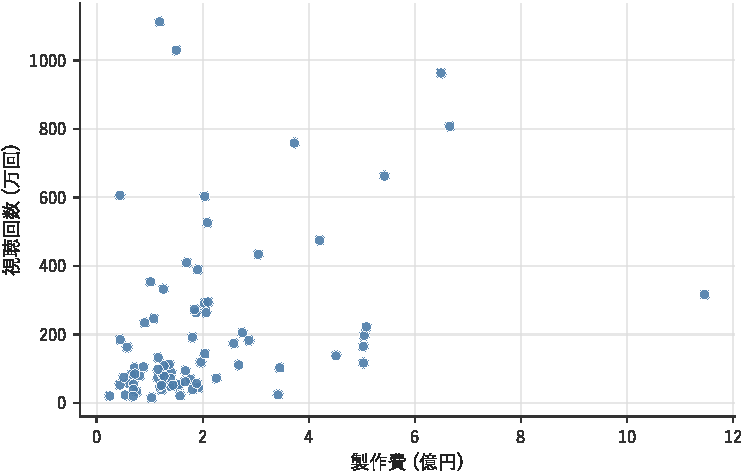
\includegraphics[width=0.7\linewidth]{../figures/output/ch03_scatter.pdf}
      \caption{製作費 (億円) を横軸に, 視聴回数 (万回) を縦軸に取り, 映画一本を一つの点で打った散布図. 縦横比は変えていない.}
      \label{fig:ch06-scatter}
    \end{figure}

    点は一直線には並んでいないが, 全体としては右上がりに見える.
    製作費の大きい映画では, 視聴回数も大きい傾向がある.
    このように, 一方が大きいものでは他方も大きい傾向があり, 散布図の点が右上がりに並ぶとき, 二つの数量には\textbf{相関}があるという.
    一方が大きいものでは他方が小さく, 点が右下がりに並ぶときも, 向きが逆の相関と呼ぶ.

    では, 製作費をかければ, そのぶん多く見られるのだろうか.
    この図からわかるのは, 製作費の大きい映画に視聴回数の大きいものが多い, ということまでだ.
    製作費の大きい映画は, 原作があるかどうかや宣伝の大きさも, 製作費の小さい映画と違っているかもしれない.
    そうだとすれば, 右上がりの一部は, 製作費ではなくそちらの違いから来ているかもしれない.

    原作の有無で映画を分けたときも, 事情は同じだった.
    原作のある映画のほうが平均視聴回数がおよそ120万回多く, 偶然とは説明しにくい差だと言えた.
    それでも, 原作があるから多く見られたとは言えなかった.
    相関があっても, 差があっても, それだけでは原因とは言えない.

    原作が原因だと言うには, 原作の有無だけが違っていて, ほかの条件がすべて揃っている二つの集まりを比べる必要があった.
    しかし, どうすればそんな集まりが手に入るだろうか.

    そもそも, ある一本の映画について「原作の効果」を確かめようとすると, 途端に行き詰まってしまう.
    その作品に本当に原作の効果があったのかを知るには, その映画を原作つきで公開したときの視聴回数と, まったく同じ映画を原作なしのオリジナル脚本で公開したときの視聴回数を比べる必要がある.
    二つの数字を引き算して差が残れば, それこそが原作の純粋な効果だと言えるはずだ.

    だが, 一本の映画を二度公開することはできない.
    見ることができるのは原作つきで世に出たほうの視聴回数だけで, 原作がなかった場合の視聴回数はどこにもないから, 一本ずつの作品について効果を直接測ることは誰にもできない.

    一本で比べられないのだとすれば, 集まりで比べるほかない.
    観測できるのは, 原作のある作品たちの平均視聴回数と, 原作のない作品たちの平均視聴回数だ.
    もしもこの二つの集まりが「原作の有無以外は同じ」であるなら, 二つの平均の差を, 原作がもたらした平均的な効果と考えて差し支えない.

  \subsection{くじで決める意味}

    前に信頼区間のところで触れた薬の治験に戻る.
    新しい薬を飲んだ集まりと, 飲んでいない集まりで血圧を比べたところ, 薬を飲んだほうが平均で 5\,mmHg 低く, 95\%信頼区間は 2\,mmHg から 8\,mmHg だった.
    このとき, 5\,mmHg という差を素直に「薬の効果」とみなしていた.
    映画では原作の効果だと言い切るのをためらったのに, なぜ治験の差なら効果だと受け取れたのだろうか.

    適切な治験では, 誰が薬を飲んで誰が飲まないかを, 医師や患者の希望ではなく, くじ引きで決める.
    このように, 集まりへの割り振りをくじなどの偶然に任せて分ける手続きを\textbf{無作為化}と呼ぶ.

    くじで分ければ, 年齢や性別, もともとの血圧の高さ, 日頃の生活習慣といったあらゆる要素が, 薬を飲むかどうかとはまったく無関係に二つの集まりへ散らばっていく.
    人数が十分に多ければ, 二つの集まりは, 薬を飲むかどうかという一点を除いて, ほかのあらゆる点でよく似た集まりになる.

    二つの集まりが薬以外の点ですでに似通っているのだから, あとから生じた血圧の差は, 薬を飲んだことによって生じた差だと考えるのが自然だ.
    だからこそ, 治験のデータから計算した標準誤差も, 信頼区間も, 検定の結果も, そのまま「薬の効果がどれくらいか」「効果が偶然のばらつきによるものではないか」の根拠として信頼することができた.

    この信用は, 差が 5\,mmHg だったという計算結果そのものから生まれたのではない.
    薬を飲む人と飲まない人をくじで分けた, という手順そのものが信用を支えている.

  \subsection{くじで分けられないデータ}

    ところが, 映画のデータに目を戻すと, 状況はまるで違っている.
    映画はくじ引きで原作つきになるかどうかが決まったわけではない.
    前章で見たように, 原作のある映画には多額の製作費や大規模な宣伝がつきやすく, 二つの集まりは最初から原作の有無以外の点でも違っている.
    平均の差の中には, 原作そのものの効果と, ほかの条件の違いがごちゃ混ぜになって入り込んでいるのだ.

    くじ引きで分けられていないデータを見るかぎり, 「原作の有無以外は同じような集まりだ」と信じるに足る根拠はどこにもない.
    それでもその差を原因によるものだと言いたいなら, 「ほかの条件に大きな違いはないはずだ」と自分で仮定を置いて比べるしかない.
    もしその仮定が外れていれば, 計算された差は原因とはまったく違うものを指し示してしまう.

    これまで見てきたように, 標本サイズを増やせば標準誤差は小さくなり, 信頼区間は狭くなって, 検定でも小さな差を有意と言えるようになる.
    だが, 標本をどれほど増やしてばらつきを小さくしても, 目に見える差と本当の効果とのあいだにある隔たりは少しも埋まらない.

  \subsection{条件をそろえて比べる}

    くじで分けることができないなら, できる手立ては何だろうか.
    一番素朴な方法は, 違っていそうな条件をそろえて比べることだ.

    たとえば, 製作費の違いが邪魔をしていると思うなら, 製作費が同じくらいの映画どうしを集めて, その中で原作のある作品とない作品の視聴回数を比べればよい.
    製作費の少ない作品の中だけで比べ, 次に製作費の多い作品の中だけで比べる, というように条件をそろえていけば, 少なくとも製作費の違いが差に混ざり込むことは防げる.
    このように, データを条件ごとにいくつかの層に分けて調べる手続きを層別と呼ぶ.

    ここで問題になっていた製作費のように, 原作の有無より先に決まっていて, 原作の有無にも視聴回数にも影響し, 見かけの差を狂わせてしまう第三の要因を\textbf{交絡}（あるいは\textbf{交絡因子}）と呼ぶ.
    条件をそろえて比べるというのは, この交絡を取り除くための作業だ.

    条件をそろえることで見え方が一変する様子は, 実際のデータでも確かめられている.
    1973年, カリフォルニア大学バークレー校の大学院で, 性別による入試の差別があるのではないかとして問題になったことがあった\footnote{Bickel, P. J., Hammel, E. A., \& O'Connell, J. W. (1975). Sex Bias in Graduate Admissions: Data from Berkeley. \textit{Science}, 187(4175), 398--404.}.
    全志願者の合格率を集計してみると, 男子の合格率は約44\%だったのに対し, 女子の合格率は約35\%で, 男子のほうが9ポイントほど高かった.
    全体だけを見れば, 男子のほうが受かりやすいように思える.

    ところが, 志願者を学部ごとに分けて合格率を計算し直してみると, まるで違う姿が現れた.
    主要な6つの学部のうち4つでは, 女子の合格率は男子と同じか, むしろ高かったのだ.
    残り2つの学部でも, 全体で出ていた9ポイントもの差は見られなかった.

    全体で9ポイントあった差は, どこへ消えてしまったのだろうか.
    実は, 学部ごとの合格率は一様ではなく, 合格率が6\%しかない狭き門の学部もあれば, 64\%もある受かりやすい学部もあった.
    そして女子の志願者は, 合格率の低い狭き門の学部に多く集まっており, 男子は合格率の高い学部に多く集まっていたのだ (\cref{fig:ch06-berkeley}).
    そのため, 学部をそろえずに全体をまとめて集計すると, 審査で男子のほうが有利に扱われているかのような差が出ていた.
    このように, 全体で見たときと分けて見たときとで差の向きが逆になったり差が消えたりする現象を, シンプソンのパラドックスと呼ぶ.

    \begin{figure}[htbp]
      \centering
      % 第6章 図6-1: バークレーの主要6学部の男女別の合格率 (上) と志願者数 (下)
% 学部別の数値は Bickel ほか (1975) の主要6学部 (R の UCBAdmissions と照合, 2026-09-27)
%   A: 男 825人 62.1%, 女 108人 82.4%   B: 男 560人 63.0%, 女  25人 68.0%
%   C: 男 325人 36.9%, 女 593人 34.1%   D: 男 417人 33.1%, 女 375人 34.9%
%   E: 男 191人 27.7%, 女 393人 23.9%   F: 男 373人  5.9%, 女 341人  7.0%
% 「全志願者」は本文の数値 (全学部: 男 約44%, 女 約35%)
\begin{tikzpicture}[font=\footnotesize]
  \begin{axis}[
    name=rate,
    width=0.82\linewidth, height=4.6cm, scale only axis=false,
    ybar, bar width=7pt,
    ymin=0, ymax=100, ytick={0,20,40,60,80,100},
    ylabel={合格率 (\%)},
    xmin=-0.7, xmax=6.7,
    xtick={0,1,2,3,4,5,6},
    xticklabels={全志願者,学部A,学部B,学部C,学部D,学部E,学部F},
    x tick label style={font=\footnotesize},
    axis x line*=bottom, axis y line*=left,
    legend style={draw=none, at={(0.98,0.98)}, anchor=north east, font=\footnotesize},
    legend image code/.code={\draw[#1] (0cm,-0.1cm) rectangle (0.3cm,0.1cm);},
    enlarge x limits=false,
  ]
    \addplot[draw=black, fill=black!15] coordinates {
      (0,44) (1,62.1) (2,63.0) (3,36.9) (4,33.1) (5,27.7) (6,5.9)};
    \addplot[draw=black, fill=black!65] coordinates {
      (0,35) (1,82.4) (2,68.0) (3,34.1) (4,34.9) (5,23.9) (6,7.0)};
    \legend{男子, 女子}
    \draw[black!40] (axis cs:0.5,0) -- (axis cs:0.5,100);
  \end{axis}
  \begin{axis}[
    at={(rate.south)}, anchor=north, yshift=-1.1cm,
    width=0.82\linewidth, height=3.2cm, scale only axis=false,
    ybar, bar width=7pt,
    ymin=0, ymax=900, ytick={0,300,600,900},
    ylabel={志願者数 (人)},
    xmin=-0.7, xmax=6.7,
    xtick={1,2,3,4,5,6},
    xticklabels={学部A,学部B,学部C,学部D,学部E,学部F},
    x tick label style={font=\footnotesize},
    axis x line*=bottom, axis y line*=left,
    enlarge x limits=false,
  ]
    \addplot[draw=black, fill=black!15] coordinates {
      (1,825) (2,560) (3,325) (4,417) (5,191) (6,373)};
    \addplot[draw=black, fill=black!65] coordinates {
      (1,108) (2,25) (3,593) (4,375) (5,393) (6,341)};
  \end{axis}
\end{tikzpicture}

      \caption{1973年のカリフォルニア大学バークレー校大学院の入試について, 主要6学部の合格率 (上) と志願者数 (下) を男女別に表した図. 左端の「全志願者」は主要6学部以外も含む全学部を合わせた合格率で, 右の6学部を合計したものではない. 学部別の数値は Bickel ほか (1975) による.}
      \label{fig:ch06-berkeley}
    \end{figure}

  \subsection{そろえてはいけない条件}

    条件をそろえれば交絡が防げるのだとしたら, 思いつく限りの条件をすべてそろえて比べればよいのだろうか.
    そろえるべきではない条件をそろえてしまうと, 今度は本物の効果を消し去ってしまうことがある.

    日常の健康を例に考えてみよう.
    運動の習慣がある人とない人で血圧を比べるとする.
    運動をすると体重が減り, その減った体重のおかげで血圧が下がっている, という関係があったとしよう.

    ここで, 「体重が違うと公平に比べられない」と考えて, 体重が同じくらいの人どうしを集めて運動の効果を比べたらどうなるだろうか.
    体重が同じ人たちの集まりの中では, 運動による「体重が減る」という効果が最初から封じ込められてしまっている.
    その結果, 運動している人と運動していない人のあいだに血圧の差は見られなくなってしまう.

    運動が効いていないわけではない.
    運動の効果は体重という通り道を通って現れていたのに, その体重をそろえてしまったために見えなくなったのだ.
    ここでの体重は, 交絡ではなく, 原因から結果へ至る道筋の途中にある.

    やっかいなのは, データの数字を見ているだけでは, ある条件が交絡なのか, それとも効果の通り道なのかを区別することはできない, という点だ.
    手元の表に並んでいる数字は, どちらの場合であってもまったく同じように見える.
    それを区別できるのは, 運動や体重や血圧が体の中でどう作用し合っているのかという, 現実の仕組みについての知識だけだ.

  \subsection{信用の根拠をどこに置くか}

    映画の分析に立ち返ってみよう.
    製作費はそろえるべきだろうか.
    原作があるから大きな製作費がつき, 宣伝も大きくなり, その結果として多く見られたのだとしたら, 製作費は交絡ではなく, 原作から視聴回数への通り道にある.
    製作費をそろえて比べることは, 体重をそろえて運動の効果を消したのと同じことになってしまう.

    どちらなのかは, 手元の数字からは決まらない (\cref{fig:ch06-paths}).
    企画が立ち上がり, 予算がつき, 宣伝され, 観客に届くまでの仕組みについての知識から考えるほかない.

    \begin{figure}[htbp]
      \centering
      % 第6章 図6-2: 製作費が交絡になる場合 (左) と通り道になる場合 (右)
% 箱と数字は同じで, 違うのは矢印の向きだけ
\begin{tikzpicture}[
    font=\small,
    box/.style={draw, rounded corners=2pt, minimum width=2.1cm, minimum height=0.75cm, fill=black!5},
    arr/.style={-stealth, thick, shorten >=1pt},
  ]
  % 左: 製作費が原作の有無と視聴回数の両方に先立つ
  \node[box] (L-cost) at (0,1.6) {製作費};
  \node[box] (L-src)  at (-1.9,0) {原作の有無};
  \node[box] (L-view) at (1.9,0) {視聴回数};
  \draw[arr] (L-cost) -- (L-src);
  \draw[arr] (L-cost) -- (L-view);
  \draw[arr] (L-src) -- (L-view);
  \node[font=\footnotesize] at (0,-0.9) {交絡になる場合};
  % 右: 原作から製作費を通って視聴回数へ
  \begin{scope}[xshift=7.2cm]
    \node[box] (R-cost) at (0,1.6) {製作費};
    \node[box] (R-src)  at (-1.9,0) {原作の有無};
    \node[box] (R-view) at (1.9,0) {視聴回数};
    \draw[arr] (R-src) -- (R-cost);
    \draw[arr] (R-cost) -- (R-view);
    \draw[arr] (R-src) -- (R-view);
    \node[font=\footnotesize] at (0,-0.9) {通り道になる場合};
  \end{scope}
\end{tikzpicture}

      \caption{製作費が交絡になる場合 (左) と, 原作の有無から視聴回数への通り道になる場合 (右) を, 矢印で表した図. 矢印は, 根元にあるものが矢印の指すものに影響することを表す. 左右で違うのは, 製作費と原作の有無を結ぶ矢印の向きだけである.}
      \label{fig:ch06-paths}
    \end{figure}

    仕組みから考えて製作費が交絡なら (左の図), 製作費をそろえて比べる必要がある.
    そろえずに比べた差には, 製作費の違いから来た分が混ざってしまうからだ.

    製作費が通り道なら (右の図), そろえると消えてしまうのは, 原作の効果のうち製作費を通って現れる分だ.
    その分まで含めた効果を知りたいなら, 製作費をそろえてはいけない.
    それを除いた効果を知りたいなら, そろえてかまわない.
    製作費をそろえずに比べたときの差は, 原作がついたことで製作費や宣伝まで大きくなった分も込みの効果だ.
    製作費をそろえて比べたときの差は, 製作費が同じだったとしたら原作の名前だけでどれだけ違うか, という効果になる.
    どちらも意味のある数だが, 同じ数ではない.
    何を知りたいのかを決めないと, そろえる条件も決まらない.

    バークレーの入試の学部も, 実は通り道のほうに近い.
    学部は性別より先に決まっていたわけではなく, 志願者が自分で選んで出願したものだ.
    性別によって志願する学部が違い, 学部によって合格率が違う, という並びは, 運動と体重と血圧の並びと同じ形をしている.
    それなら, 学部をそろえて比べたのはまずかったのだろうか.

    当時問題になっていたのは, 審査で女子が不利に扱われていないか, ということだった.
    審査は学部ごとに行われるので, 審査での扱いを確かめるなら, 同じ学部の志願者どうしで比べるのが筋だ.
    学部をそろえて比べたのは, 知りたいことに合っていたのだ.
    この件を調べた研究者たちも, 審査で女子が不利に扱われていたとは言えず, 全体の差は女子が狭き門の学部に多く出願していたことから生じた, と結論している.

    一方, 女子の志願が狭き門の学部に集まっていること自体を問題にするなら, 全体の9ポイントの差にも意味がある.
    女子であることが, 学部選びまで含めて合格の機会をどれだけ狭めているかを表す数になるからだ.
    ただし, その差を生んだのは審査ではなく, どの学部に志願するかの偏りと, その偏りの背景にある事情だ.

    それでもなお, くじ引きで分けた治験から得られた差と, ほかの条件をそろえて比べた映画の差とでは, 置いている信用の種類が根本から異なっている.
    治験の差は, くじ引きで分ければ二つの集まりが揃うからこそ, その手順の確かさを根拠にして信じることができた.
    一方, 映画のようにくじで分けられないデータから得られた差は, 「必要な条件はすべてそろえたはずだ」という仮定に支えられているにすぎない.
    原因を確かめるにはほかの条件がすべて揃っている集まりが要ると言ったが, 通り道になっている条件までそろえれば本物の効果まで消えてしまうことがあるので, 「すべて」は言いすぎだった.
    残りの条件をすべてそろえることも, 実際にはできない.
    できるのは, 差を狂わせそうな条件を思いつくかぎり挙げ, そのうち測れたものをそろえることだけだ.
    もし見落とした条件が一つでも残っていれば, 導き出された結論はいつでも揺らぎうるのだ.

  \begin{mybox}{ここまででわかったこと}
    四段階の四つ目「仮定を確かめて判断する」.

    \textbf{この章で言えるようになったこと}: 製作費と視聴回数に相関があっても, 製作費をかけたから多く見られたとは言えない.
    治験の $5\,\mathrm{mmHg}$ の差を薬の効果と考えられたのは, 飲む人と飲まない人をくじで分けたからだった.
    くじで分けていない映画の約120万回の差を原作の効果と言うには, ほかの必要な条件がそろっているという仮定が要る.

    \textbf{まだ言えないこと}: 比べる作品の条件をそろえても, そもそも手元の80本が人気作ばかりだったらどうだろうか.
    この80本から作品全体のことが言えるかは, まだ確かめていない.

    \textbf{前の章の見方がどう変わったか}: 本数を増やせば差の区間は狭くなるが, それだけでは原作の効果に近づかない.
  \end{mybox}


\newpage

% 第7章 = 第6段「確率の意味は, 調査から報告までの何を繰り返すかで決まる」
\section{前提を確かめる：バイアス}

  \subsection{集め方の偏りと人数の限界}

    前章では, 原作の有無による差が本物の効果なのかを調べるために, 条件をそろえて比べる方法を考えた.
    くじで分けられないデータから差の理由を言うには, 「ほかの条件に大きな違いはないはずだ」という仮定に頼るしかなかった.

    だが, その話の足元には, もっと手前で置いたきりの前提が残っている.
    標本を取り直せば平均が散らばるという話をしたときから, 手元の80本は「対象作品全体から大きな偏りなく抽出された標本である」として扱ってきた.
    区間を作っても, 差を検定しても, 条件をそろえても, 出てきた結果を作品全体の話として言えるのは, この前提があってこそだった.
    もし集めてきたデータが最初から偏っていたとしたら, ここまでの計算はどうなってしまうだろうか.

    極端な場面を考えてみよう.
    たとえば日本に住む有権者全体の意見を知りたいのに, 平日の昼に渋谷駅にいた人だけに話を聞いたとする.
    平日の昼間に渋谷駅を歩いている人たちと, 有権者全体とでは, 年齢層も職業も日頃の暮らしもまるで違うはずだ.
    この方法で10万人の意見を集めたとしよう.
    10万人といえば途方もない規模だが, いくら人数を積み上げても, 平日の昼に渋谷駅にいなかった人たちの声は最初から最後までゼロのままだ.

    人数を増やすと, 標準誤差の分母にある $\sqrt{n}$ が大きくなるため, 計算される信頼区間はどこまでも狭くなっていく.
    一見すると, 推定の精度がどんどん上がっているように思えるかもしれない.
    しかし, 区間の中心である標本平均が近づいていく先は, 知りたかった有権者全体の平均ではなく, 「平日の昼に渋谷駅にいた人たち」の平均でしかない (\cref{fig:ch07-biased-n}).
    中心そのものがずれているのだから, 区間をどれほど狭く絞り込んでも, 本当に知りたい値から外れた場所を精密に指し示し続けるだけになってしまう.

    \begin{figure}[htbp]
      \centering
      % 第7章 図7-1: 偏った集め方のまま人数を増やしたときの信頼区間 (模式図, 目盛りなし)
% 区間の半分の長さは 1/sqrt(n) に比例させた: 100人 3.0, 1000人 0.95, 10万人 0.095
\begin{tikzpicture}[x=0.75cm, y=1cm, font=\footnotesize]
  % 知りたい値と, 偏った集まりの平均
  \draw[densely dashed] (0,-0.3) -- (0,3.3);
  \draw[densely dotted, thick] (6,-0.3) -- (6,3.3);
  \node[above, align=center] at (0,3.3) {有権者全体の平均};
  \node[above, align=center] at (6,3.3) {平日の昼に渋谷駅に\\いた人たちの平均};
  % 区間
  \foreach \y/\c/\h/\lab in {2.4/5.5/3.0/100人, 1.4/6.3/0.95/1000人, 0.4/5.97/0.095/10万人} {
    \draw[line width=2.2pt, black!55] ({\c-\h},\y) -- ({\c+\h},\y);
    \draw[thick] ({\c-\h},\y-0.14) -- ({\c-\h},\y+0.14) ({\c+\h},\y-0.14) -- ({\c+\h},\y+0.14);
    \fill (\c,\y) circle (2.2pt);
    \node[left] at (-0.6,\y) {\lab};
  }
\end{tikzpicture}

      \caption{平日の昼に渋谷駅にいた人だけに話を聞く方法で, 聞く人数を100人, 1000人, 10万人と増やしたときの信頼区間の模式図 (目盛りは付けていない). 黒い点は区間の中心の標本平均. 破線は有権者全体の平均, 点線は平日の昼に渋谷駅にいた人たちの平均の位置を示す. 区間の長さは, 人数の平方根に反比例するように描いた.}
      \label{fig:ch07-biased-n}
    \end{figure}

    同じ手順で作った区間には100回に95回ほど母平均が入る, という約束が成り立つのは, 標本が知りたい母集団全体から偏りなく選ばれているときだけだ.
    もし集め方が最初から偏っていれば, 同じ調査をどれほど繰り返したところで, 100回に95回入るのは母集団全体の平均ではなく, 偏って集められた集まりの平均である.
    このように, 標本を集める手順そのものに偏りがあることを\textbf{サンプリングバイアス}と呼ぶ.

    選挙の前に, ネットで「誰に投票しますか」と尋ねる投票が行われ, 10万票が集まって, 候補Aが7割の票を取ったとする.
    同じころ, 有権者から無作為に選んだ1000人に聞いた調査では, 候補Aは32\%と出ていた.
    実際の選挙では, 候補Aの得票は30\%だった.
    当たっていたのは, 100分の1の人数しか聞いていない調査のほうだ.

    1000人に聞けば, 世論調査の支持率で計算したとおり, $\pm 3$ポイントほどの幅がつく.
    32\%の上下3ポイントには, 30\%がちゃんと入っている.
    同じ計算を10万票に当てはめると, 幅は $\pm 0.3$ポイントほどまで縮む.
    その狭い区間が, 実際の30\%から40ポイントも離れたところにあった.

    ネットで票を入れたのは, 自分から投票しに来た人たちだけだった.
    票数が増えるほど, その人たちの意見を精密に指すようになるだけで, 有権者全体には近づかない.
    \cref{fig:ch07-biased-n} でいえば, 10万票の7割は, 点線の位置を短い区間で指していたことになる.

    1000人の調査とネットの投票を分けたのは, 人数ではなく, 誰の声が集まったかだった.
    偏りは, 聞く相手を選ぶ前から入り込んでいることもある.
    映画80本にも, それが起こりうる.
    80本を選んだ元の一覧に並んでいるのは, いまそのサービスで配信されている作品だ.
    公開から30日間ほとんど見られず, その後に配信を終えた作品があったとしても, 一覧にはもう載っていない.
    母集団をこれまでどおり配信されている作品全体とするなら, これは偏りではない.
    消えた作品は, はじめから母集団に入っていないからだ.
    だが, 知りたいのが「映画は配信でどれくらい見られるものか」だったらどうだろう.
    見られなかった作品ほど配信を終えやすいのなら, 一覧そのものが, これまでに配信された作品全部より, 見られた作品のほうへ寄っていることになる.
    一覧から80本を選ぶ手順をどれほど丁寧にしても, 選ぶ前に一覧から消えた作品は80本の中に入りようがない.
    同じ一覧でも, 知りたい全体が違えば, 偏っているかどうかも違ってくる.

    途中で消えずに残ったものだけが手元に集まって生じるこの偏りを\textbf{生存者バイアス}と呼ぶ.
    成功した経営者の習慣を集めた本に, 早起きや毎朝の運動といった共通点が並んでいるのも同じ形だ.
    同じ習慣を続けていても事業に失敗した人は本に取り上げられないので, その習慣が失敗した人にも同じくらい多かったかどうかは, どこにも書かれていない.

  \subsection{数字は何を測っているか}

    集め方に偏りがなかったとしても, 手元にある数字そのものが何を測っているのか, という問題が残っている.

    ここまで映画80本について調べてきたのは, 1本あたりにならすとどれくらい見られているか, 原作の有無で平均視聴回数に差があるか, だった.
    どちらも視聴回数についての疑問で, 視聴回数を数えているかぎり, ずれはない.

    ところが, 出てきた数を見て「原作のある作品のほうが面白い」「こちらのほうが質が高い」と言いたくなる.
    そこで一歩はみ出してしまう.

    視聴回数が数えているのは, 再生ボタンが押されて動画が始まった回数だ.
    見始めて5分で止めた人の1回も, 最後まで見て二度見返した人の1回も, 同じ「1回」として入っている.
    面白さを直接数えることはできないので, 数えられるものを数えている.

    通販サイトの星の数でも同じことが起きている.
    製品の品質を知りたいと思って星の数を眺めるが, 星1つがついていても, その理由は製品そのものではなく, 配送が予定より遅れたことへの不満かもしれない.
    逆に, 期待がそれほど高くなかったために星5つがついていることもある.
    星の平均を見るときに一人ひとりの評価が均等にならされてしまうことは確かめたが, ならされる前の一つひとつの星にも, 「製品の良し悪し」以外の事情が混ざり込んでいる.

    平均の計算も, 信頼区間も, 検定も, すべて「視聴回数」や「星の数」という手元の数字については正しく行われている.
    問題があるとしたら, 出てきた数字をいつの間にか「面白さ」や「商品の質」そのものの話として解釈してしまうところにある.

    映画の本数をいくら増やしたところで, 視聴回数が「再生が始まった回数」であることに変わりはなく, 知りたいものと測っているものとのずれは縮まらない.

    このずれは, 手元のデータをいくら眺めていても見えてこない.
    数字の計算を見るのではなく, その数字がどのように数えられ, 何を聞いて記録されたものなのかという, データが作られた経緯を確かめるしかない.

  \subsection{選ばれた結果と珍しさの意味}

    集め方にも, 測っているものにも問題がなかったとしても, もう一つ別の場所から数字の解釈を狂わせる問題が入り込む.
    計算された結果の選び方だ.

    ここに1枚のコインがあるとする.
    このコインを100回投げてみたところ, 表が62回出た.
    表と裏が半分ずつ出るふつうのコインなら, 表が出る回数の期待値は50回だ.
    検定の枠組みに沿って, 「このコインは表と裏が同じ確率で出る」という帰無仮説を立て, 有意水準5\%で検定してみる.
    計算される$p$値はおよそ0.02となり, 0.05を下回る.
    帰無仮説は棄却され, 表と裏の出方に偏りがある, つまり「このコインには細工がありそうだ」という結論になる.
    前章までの話のとおりで, 筋の通った結論だ.

    実は, 手元にはコインが最初から20枚あった.
    その20枚のコインをすべて100回ずつ投げ, 20回分の検定を行った.
    残りの19枚は, ひとつも有意にはならなかった (\cref{fig:ch07-coins}).
    そして, $p$値が0.05を下回ったたった1枚のコインだけを, 先ほどのように取り出して見せたのだ.
    1枚1枚の計算には何の誤りもない.

    \begin{figure}[htbp]
      \centering
      % 第7章 図7-2: 細工のないコイン20枚を100回ずつ投げたときの表の回数 (例示用のデータ)
% 19枚は二項分布 (100回, 0.5) から 40〜60回の範囲で乱数生成 (seed 20260927), 13枚目を62回に固定
% 両側の二項検定で有意水準5%を下回るのは 39回以下か61回以上 (60回で p=0.057, 61回で p=0.035, 62回で p=0.021)
\begin{tikzpicture}[font=\footnotesize]
  \begin{axis}[
    width=0.8\linewidth, height=5.2cm,
    xmin=0.2, xmax=20.8, ymin=30, ymax=70,
    xtick={1,5,10,15,20}, ytick={30,40,50,60,70},
    xlabel={コインの番号}, ylabel={表の回数},
    axis x line*=bottom, axis y line*=left,
    clip=true,
  ]
    % 有意になる範囲
    \fill[black!12] (axis cs:0.2,60.5) rectangle (axis cs:20.8,70);
    \fill[black!12] (axis cs:0.2,30) rectangle (axis cs:20.8,39.5);
    \draw[densely dashed, black!60] (axis cs:0.2,50) -- (axis cs:20.8,50);
    \addplot[only marks, mark=*, mark size=2.3pt, mark options={fill=white, draw=black}] coordinates {
      (1,48) (2,43) (3,43) (4,48) (5,47) (6,52) (7,55) (8,50) (9,56) (10,42)
      (11,43) (12,50) (14,53) (15,55) (16,42) (17,51) (18,48) (19,57) (20,45)};
    \addplot[only marks, mark=*, mark size=2.8pt, mark options={fill=black, draw=black}] coordinates {(13,62)};
    \node[font=\footnotesize, anchor=south] at (axis cs:10.5,63.5) {有意になる範囲 (61回以上)};
    \node[font=\footnotesize, anchor=north] at (axis cs:10.5,36.5) {有意になる範囲 (39回以下)};
  \end{axis}
\end{tikzpicture}

      \caption{コイン20枚をそれぞれ100回投げたときの, 表の出た回数. 例示用に作ったデータで, 13枚目 (黒い点) を62回としている. 横軸はコインの番号, 縦軸は表の回数. 灰色の範囲は, 表と裏が同じ確率で出るという帰無仮説を有意水準5\%で検定したときに有意になる回数 (39回以下と61回以上), 破線はその帰無仮説のもとでの期待値50回を示す.}
      \label{fig:ch07-coins}
    \end{figure}

    しかし, このコインには本当に細工があると言っていいのだろうか.
    有意水準5\%という基準を思い出してみよう.
    これは, 「細工のないふつうのコインであっても, 20回に1回ほどは偶然で有意になってしまう」という誤りを認める約束だった.
    ということは, まったく細工のない公平なコインを20枚集めてきて同じ実験をすれば, そのうちのどれか1枚くらいは, 偶然だけで有意になってしまっても何の不思議もない.

    細工のないコインを20枚投げたとき, 少なくとも1枚が偶然有意になってしまう確率は, 次のように計算できる.
    有意水準どおりに, 1枚が偶然有意になる確率を5\%と置いてみる.
    コイン1枚が有意にならない確率は $0.95$ だから, 20枚すべてが有意にならない確率は $0.95^{20}$ になる.
    その裏返しとして, 20枚のうちどれか1枚でも有意になる確率は,
    \[
      1 - 0.95^{20} \approx 0.64
    \]
    とおよそ64\%になる.
    3回に2回ほどの割合で, 細工など何もないふつうのコインの集まりから「有意な偏り」が勝手に生み出されてしまうわけだ.

    1枚だけを投げて有意になるのは, 確かに珍しい出来事だ.
    しかし, 20枚投げてその中から有意になったものだけを拾い上げるなら, それは少しも珍しいことではない.
    その1枚について計算された$p$値の数字は少しも変わっていないのに, 「珍しいことが起きた」という言葉の重みがまるで違ってしまう.

    このように, 望ましい結果が出るまで条件や対象を変えて分析を繰り返し, 有意になったものだけを取り出す行為を\textbf{$p$ハッキング}と呼ぶ.
    そうならないように, データを見る前に, 「どの比較を行うのか」「何を試すのか」をあらかじめ決めておく.
    結果を見てから都合よく動かさないために有意水準を事前に決めておいたのと同じように, 分析の対象そのものも事前に固定しておく必要がある.
    そして, 試したものは, 有意にならなかったものも含めて全部を示す.
    データを眺めていて傾向に気づくのは悪いことではなく, 確かめてみる値打ちのある見当が手に入ったということだ.
    ただ, 気づいたのと同じデータでその珍しさを測れば, 20枚のコインから有意な1枚を拾うのと変わらない.
    確かめるには, 新しくデータを集めて測り直す.

    選んだことで数字の意味が変わるのは, 検定を何度も試したときだけではない.
    ある学校で, 試験の成績が下のほうだった生徒たちを選んで, 特別に指導したとする.
    次の試験では, その生徒たちの平均点が上がった.
    指導の効果が出たように見える.
    だが, 選んだのは一回の試験で下のほうにいた生徒だ.
    標本を取り直せば平均が動いたように, 一人の点数も, 同じ生徒が試験を受け直せば上下する.
    下のほうにいた生徒の中には, たまたまその回の出来が悪かった生徒が混ざっている.
    そうした生徒は, 指導がなくても, 次の回にはふだんの点数のあたりに戻ってくる.

    そのため, 選んだ生徒たちの平均点は, 指導をしなくても前の回より上がりやすい.
    下のほうから選んで測り直すと, ばらつきだけで戻る分が, 指導の効果のように見えてしまうのだ.
    このように, 一回の結果で選んだ集まりを測り直したとき, その平均が全体の平均のほうへ戻っていくことを\textbf{平均への回帰}と呼ぶ.
    20枚のコインと同じで, 点数の計算はどこも間違っていないのに, 誰を選んで測り直したかで, 上がった点数の意味が変わってしまう.
    指導の効果を確かめたいなら, 薬の治験と同じように, 選んだ生徒をくじで二つに分け, 片方だけを指導すればよい.
    どちらの側にも, たまたまその回が悪かった生徒が同じように混ざるので, 戻る分は両方に同じように出るはずだ.
    それでも二つの平均点に差が残れば, その差は指導によるものと考えてよく, 偶然のばらつきで説明できるかどうかは, 前の章までと同じ手順で確かめられる.

  \subsection{繰り返しているものの正体}

    この本では最初から, 一回きりのデータにとらわれず, 「もし同じ調査を何度もやり直したら」という想像を土台にして進んできた.
    標本を取り直せば平均が散らばることを確かめ, 同じ手順で作った区間には100回に95回ほど母平均が入ると言い, 差が本当にないときに検定を繰り返せば有意になるのは20回に1回ほどだと約束した.

    しかし, やり直すといっても, やり直しているものは一つではなかった.
    区間の約束でやり直しているのは, 全体から標本を選ぶところだ.
    全体から偏りなく選ぶことを何度も繰り返すと考えるから, 「100回に95回」は全体の平均についての話になる.
    くじで分けたときにやり直しているのは, 目の前に集まった人たちを二つに分けるところだ.
    分け直すたびに顔ぶれは入れ替わるが, 人数が十分に多ければ, 薬や指導のほかの点では, どちらの側にも同じような人が入る.
    だから, 残った差を薬や指導の効果だと言える.
    偏りなく集めれば, 結果を全体の話として言える.
    くじで分ければ, 差を原因の話として言える.
    この二つは別のことだ.

    さきほどの生徒たちは, 試験の下のほうから選んだのだから, 学校全体から偏りなく集めた集まりではない.
    それでも, くじで分ければ, 選ばれた生徒たちについては指導の効果があったかどうかを確かめられる.
    ただ, 同じ指導が学校のほかの生徒にも同じように効くかどうかまでは言えない.
    そこまで言うには, 集め方のほうが要る.
    治験も同じだ.
    くじが保証してくれるのは, 治験に参加した人たちの中で薬が効いたかどうかまでだ.
    参加していない人にも同じように効くかどうかは, 参加した人たちがどう集まったかにかかっている.

    100回に95回, あるいは20回に1回という確率が何を意味しているのかは, 自分が何を繰り返すことにしているかによって決まる.
    それは数式に数字を入れて計算することだけでなく, どこからデータを集めてどう分け, その数字が何を測っていて, 何を試してどの結果を見せているのかという, 調査や分析の進め方そのものを含んでいる.

  \subsection{条件を確かめて語る}

    映画80本の分析に戻って, 手元にある結果をもう一度見直してみよう.

    手元のデータから導き出された事実は, 筋道としてははっきりしている.
    80本の平均視聴回数は $209.4$ 万回で, 母平均の95\%信頼区間はおよそ156万回から263万回だった.
    そして原作のある作品とない作品とでは平均して120万回ほどの差があり, その差は偶然のばらつきだけでは説明しにくいものだった.

    しかし, この結果を説明するには, 計算の正しさを示すだけでは足りない.
    その数字がどんな前提の上に立っているのかを, 自分の手で確かめておく必要がある.

    まず確かめるべきなのは, この80本の結果をどの全体の話として言うのか, という点だ.
    80本を選んだ一覧には, 見られずに配信を終えた作品が載っていなかった.
    一覧から偏りなく80本を選んでいれば, 計算した区間は, いま配信されている作品全体の平均についての区間だと言える.
    だが, これまでに配信された作品全部の話にしようとすると, 消えた作品が抜けている分, 80本全体の平均は高めに出ているかもしれないし, 原作の有無による差も違っていたかもしれない.

    あわせて確かめるべきなのは, 原作の有無という比較が, 最初からそれだけを調べるつもりで選ばれたのか, という点だ.
    もし, 映画のジャンルや公開月, 上映時間や主演俳優の年齢など, 何十通りもの切り口で視聴回数を手当たり次第に比べ, その中でたまたま$p$値が0.05を下回ったのが「原作の有無」だったのだとしたらどうだろうか.
    それは20枚のコインを投げて有意になった1枚だけを取り出したのとまったく同じで, 偶然のばらつきを拾い上げたにすぎないかもしれない.
    分析を始める前から「原作の有無で差があるか」という一点を確かめようとしていたと分かってはじめて, $p$値の小ささはそのままの重みを持つ.

    いま配信されている作品の一覧から偏りなく選んだ80本なら, 1本あたりの平均視聴回数は209.4万回で, 配信中の作品全体の平均はおよそ156万回から263万回と見積もってよい.
    原作の有無を最初から比べるつもりだったのなら, 原作のある作品のほうが平均して120万回ほど多く見られているという差も, 偶然のばらつきだけでは説明しにくい.
    配信を終えた作品まで含めた, これまでに配信された作品全部の話や, 原作があれば視聴回数が増えると言い切ることは, この80本からはできない.
    それでも, この一覧から集め, この比較を先に決めて分析したのなら, ここまではっきり言える.

  \begin{mybox}{ここまででわかったこと}
    四段階の四つ目「仮定を確かめて判断する」.

    \textbf{この章で言えるようになったこと}: これまでに配信された作品全部の話をするなら, 見られずに配信を終えた作品は一覧に残らないので, 80本は見られた作品のほうへ寄っているかもしれない.
    20枚から有意な1枚を選んだコインは, $p$値が約 $0.02$ でも珍しくない.
    下のほうから選んだ生徒の点数は, 指導がなくても測り直せば上がりやすい.

    \textbf{まだ言えないこと}: この80本の視聴回数だけでは, 原作をつければ作品がどれだけ面白くなるかまでは言えない.

    \textbf{前の章の見方がどう変わったか}: 比べる二つの集まりの条件だけでなく, どこから集め, 何を数え, どの結果を選んだかも確かめる必要があった.
    「同じ手順を繰り返す」には, 計算の前後でしていたことまで入っていた.
  \end{mybox}


\newpage

\appendix
\section{平均と期待値}

    \cref{thm:mean-expectation}の「ランダムに取り出す」とは, $n$ 個ある位置のどれもが同じ確率 $1/n$ で選ばれる, という意味である.

    まず位置で数えてみる.
    $i$ 番目の位置が選ばれる確率は $1/n$ で, そのとき $X$ は $x_i$ になる.
    期待値は値にその確率をかけて足したものなので,
    \[
      E[X] = \sum_{i=1}^{n} x_i \cdot \frac{1}{n} = \frac{1}{n}\sum_{i=1}^{n} x_i = \bar{x}
    \]
    となる.

    少し気になるのは, 同じ値がいくつも並んでいる場合だ.
    期待値の定義では, 異なる値ごとに「値 × その値が出る確率」を足すのだった.
    そこで, 異なる値 $v$ のそれぞれについて, $v$ が並んでいる位置の個数を $c_v$ とする.
    $X = v$ になるのは $c_v$ 個の位置のどれかが選ばれたときなので, $P(X = v) = c_v/n$ である.
    よって
    \[
      E[X] = \sum_{v} v \cdot \frac{c_v}{n} = \frac{1}{n}\sum_{v} c_v v
    \]
    となる.
    $c_v v$ は同じ値 $v$ を $c_v$ 回足したものだから, 右辺は $x_1$ から $x_n$ までを同じ値どうしでまとめてから足しているだけである.
    まとめ方を変えても合計は変わらないので, これも $\frac{1}{n}\sum_{i=1}^{n} x_i$ に等しく, 位置で数えたときと一致する.

    商品Bの20件で確かめてみる.
    1点が5件, 5点が15件なので, $P(X=1) = 5/20$, $P(X=5) = 15/20$ である.
    \[
      E[X] = 1 \cdot \frac{5}{20} + 5 \cdot \frac{15}{20} = \frac{5 + 75}{20} = 4.0
    \]
    となり, 本文で求めた平均4.0と一致する.


\end{document}
